
\documentclass[conference]{IEEEtran}
\usepackage{blindtext, graphicx}
\usepackage{cite}
\usepackage{lipsum}
\usepackage{comment}
\usepackage{hyperref}
\usepackage{multirow}
\newcommand{\mailtodomain}[1]{\href{mailto:#1@masdar.ac.ae}{\nolinkurl{#1}}}
\ifCLASSINFOpdf

\else

\fi

\hyphenation{op-tical net-works semi-conduc-tor}


\begin{document}
%
% paper title
% can use linebreaks \\ within to get better formatting as desired
\title{A Two-Stage Comparative Life Cycle Assessment of Paper-Based and Digital Business Cards}


% author names and affiliations
% use a multiple column layout for up to three different
% affiliations
%\author{\IEEEauthorblockN{Michael Opolot}
%\IEEEauthorblockA{Mechanical Engineering\\%Department of \\Mechanical Engineering\\
%Masdar Institute\\
%Masdar, Abu Dhabi\\
%Email: mopolot@masdar.ac.ae}%http://www.michaelshell.org/contact.html}
%\and
%\IEEEauthorblockN{Kartoshka Yaqub}
%\IEEEauthorblockA{Computing and Information Science\\
%Masdar Institute \\
%Email: wyaqub@masdar.ac.ae}
%\and
%\IEEEauthorblockN{Aregushka Artoshka}
%\IEEEauthorblockA{KARTOSHKA Academy\\
%San Potato, California 96678-2391\\
%Telephone: (800) 555--1212\\
%}}


% conference papers do not typically use \thanks and this command
% is locked out in conference mode. If really needed, such as for
% the acknowledgment of grants, issue a \IEEEoverridecommandlockouts
% after \documentclass

% for over three affiliations, or if they all won't fit within the width
% of the page, use this alternative format:
% 


\author{
    \IEEEauthorblockN{Areg Karapetyan\IEEEauthorrefmark{1}, Waheeb Yaqub\IEEEauthorrefmark{4}, Aram Kirakosyan\IEEEauthorrefmark{3}}
    \IEEEauthorblockA{Department of Electrical Engineering and Computer Science\\
    Masdar Institute of Science and Technology\\
    Abu Dhabi, UAE
    \\\{\IEEEauthorrefmark{1}\mailtodomain{akarapetyan}, \IEEEauthorrefmark{4}\mailtodomain{wyaqub}, \IEEEauthorrefmark{3}\mailtodomain{akirakosyan}\}@masdar.ac.ae}

}


% use for special paper notices
%\IEEEspecialpapernotice{(Invited Paper)}




% make the title area
\maketitle


\begin{abstract}
Information and digital communication technologies are playing an important role in shaping the future of communities and societies. Identifying the environmental impacts and burdens of digital products and services is helpful for taking sustainable decisions. This article introduces the findings of a comparative life cycle assessment of two business card options: a smartphone software and a corresponding paper-based alternative. Life cycle burdens of the production and exchange of business cards were compared and contrasted for both systems. Furthermore, as far as we have been able to determine, there has been no study evaluating the environmental impacts of software-based and paper-based business cards. Given the prevalence and multifunctionality of digital devices and services, this paper identifies and evaluates environmental impact categories as well as the total energy consumption, Green House Gas (GHG) emissions, toxic releases of two systems by conducting a two-stage life cycle assessment with alternating functional units. The results revealed that, for a small scale functional unit, paper-based business card system had less environmental impact and energy demand, specifically, life cycle energy consumption and environmental impacts of the paper-based business card system were nearly 3.5 times and 15\% less than those of the digital business card system respectively. Whereas for a large scale (real world scenario) functional unit, the digital business card system were more environmentally friendly and economical in terms of energy consumption. By comparing these two systems, this paper could serve businesses and consumers as a basis for considering environmental consequences and energy depletion regarding two business card options.
\begin{comment}
Information and digital communication technologies are playing an important role in shaping the future of communities and societies. Identifying the environmental impacts and burdens of digital products and services is helpful for taking sustainable decisions. This article introduces the findings of a comparative life cycle assessment of two business card options: a smartphone software and the corresponding paper-based alternative. Environmental impacts of the production and exchange of business cards were compared and contrasted for both systems. Furthermore, as far as we have been able to determine, there has been no study evaluating the environmental impacts of  
software-based and paper-based business cards. Given the prevalence and multifunctionality of digital devices and services, this paper evaluates the total energy consumption, Green House Gas (GHG) emissions, toxic releases and other environmental impacts of two systems by conducting a two-stage life cycle assessment with alternating functional units. The results revealed that for a small scale functional unit, the paper-based business card system had less environmental impact and energy consumption, whereas for a large scale (real world scenario) functional unit, the digital business card system was more environmentally friendly and economical in terms of energy depletion. By comparing these two systems, this paper could serve businesses and consumers as a basis for considering environmental consequences and energy depletion regarding two business card options. 
\end{comment}

\end{abstract}
% IEEEtran.cls defaults to using nonbold math in the Abstract.
% This preserves the distinction between vectors and scalars. However,
% if the journal you are submitting to favors bold math in the abstract,
% then you can use LaTeX's standard command \boldmath at the very start
% of the abstract to achieve this. Many IEEE journals frown on math
% in the abstract anyway.

% Note that keywords are not normally used for peerreview papers.
\begin{IEEEkeywords}
Life Cycle Assessment, Information and Communication Technologies, Internet, Environmental Impact, Input-Output LCA, Printed Business Cards, Digital Business Cards. 
\end{IEEEkeywords}


% For peer review papers, you can put extra information on the cover
% page as needed:
% \ifCLASSOPTIONpeerreview
% \begin{center} \bfseries EDICS Category: 3-BBND \end{center}
% \fi
%
% For peerreview papers, this IEEEtran command inserts a page break and
% creates the second title. It will be ignored for other modes.
\IEEEpeerreviewmaketitle


\section{Introduction}

Human originated impacts on climate variation, increased consumption of natural resources, specifically fossil fuels, as well the as harmful consequences of industrial pollution have drawn global consciousness to the concepts of sustainability -welfare of future generations and life cycle thinking, which significantly constrained not only industrial and commercial sectors of the global economy, but also routine activities in terms of energy and resource consumption and environmental footprint. At the same time, thanks to exponential growth of the World Wide Web (Internet) and the explosive advances in digital technologies over the past decade, the information and communication technologies (ICT) sector is revolutionizing and modifying the pathways of both human activity and the global economy. One of the most distinguishable transitions is that from paper to digital. Nowadays, paper based products and services such as invoices, billing systems, teaching, books, magazines and newspapers, advertising, diaries, business cards and office documentation all have their digital alternatives.

Comparative analysis of the environmental impacts of traditional paper based products and their corresponding ICT enabled digital counterparts has been a subject of a  considerable body of research studies, including but not limited to comparison of digital and paper media, digital and print libraries, electronic and paper billing methods, printed and electronic teaching aids, printed newspaper, Internet newspaper and TV broadcast, online and paper based telephone directories, e-mail and traditional postal mail service, as well as printed scholarly books and e-book reading devices \cite{Bull201410, 6360455, enroth2009, zurkirch2000, kozak2003,hischier2003multifunctional }. Whereas, despite nowadays wide usage and high popularity of business cards\footnote{A card bearing business information about a company or individual} intended for promoting a person or business, to the best of our knowledge, information and data associated with the environmental effects and energy consumption during creation and usage of paper based business cards(PBC)\footnote{White or full color paper stock having printed text and/or image(s) representing information about a business or person} and digital business cards (DBC)\footnote{A digital data containing information regarding a business or person stored in a local storage of a smartphone and accessible as a visualization} have not been well studied and quantified. In fact, according to CNN report and a number of Internet resources, in 2012 the annual number of printed business cards was estimated to be 10 billion.

On the one hand, various research studies indicate that impressive rates of growth of technological advances and innovations have empowered the ICT sector with enough potential for reducing global energy and resource consumption and GHG emissions  \cite{10046363,924525, 6360455}. According to \cite{3758490, 7282419} technical reports, further modified ICT applications could save up to 7.8 GtCO2e, or 15\% of global CO2 equivalent emissions by 2020. From an economic perspective, this is synonymous to approximately \$743 billion of cost savings in terms of energy conservation.

On the other hand, the ICT sector itself challenges the environment and global energy reserves, which in combination with the tremendous rate of growth of the ICT sector contributes to the growing concerns about environmental impacts of ICT. A number of studies aimed at modeling, evaluating and identifying the direct and indirect influence of ICT applications on the global economy and environment, show that, because of its intermittent, extremely vague and interrelated nature, it is possible that ICT could have undesirable effects on the environment  \cite{Hilty20061618, 6083606, Bull201410}. According to \cite{7282419}, a typical Google search performed from a desktop computer can produce about 7g of CO2 per search. Considering that on average, there are 3.5 billion Google searches per day, the resulting aggregate CO2 emissions only from these searches amounts to 24.5 KtCO2 per day, which is equivalent to the CO2 emissions from 2 million second generation 2004 Toyota Prius vehicles having a run of 100 km (based on the assumption that second generation 2004 Toyota Prius vehicle emits 118.84 $\frac{g}{km}$ \cite{6728838}). In 2002, the ICT sector's total contribution to global GHG emissions was estimated to be 530 MtCO2e, whereas in 2007, the emissions increased to 620 MtCO2e (1.3\% increase) of the cumulative global GHG emissions. It has been forecasted that by 2020, ICT could cause GHG emissions of the order of 1.43 GtCO2e  \cite{malmodin2013future, 3758490}.

ICT have become an inseparable component of our personal and professional lives, and have a promising potential for environmental footprint abatement. Nevertheless, the ever increasing rate of growth of ICT applications and the aforementioned calculations demonstrate that quantifying and evaluating the direct environmental footprint of ICT applications is of crucial importance in terms of environmental preservation. Life Cycle Assessment (LCA), a widely used concept and technique for evaluating the environmental effects of a product or activity holistically has been considered in this study. LCA study analyzes the environmental aspects and potential environmental impacts throughout a product's life cycle that is, from raw material acquisition through production, use, end-of-life treatment, recycling and final disposal (i.e. cradle-to-grave)" \cite{ISO140402006}.

This study, by means of LCA methodology, provides the findings of a comprehensive and non-discriminatory cradle-to-grave comparison and examination of environmental aspects and energy utilization of business cards in digital and traditional (paper) formats. The contributions and findings of this paper illustrate businesses and consumers with viable and sufficient information to consider the relative environmental consequences, as well as the energy depletion corresponding to each business card option.

\begin{comment}
as shown in Figure \ref{fig:cradleToGrave}. LCA is a relatively recent well defined and transparent technique used to estimate environmental burdens generated all through the lifetime of a product, service or process within the system defined boundary. Environmental impacts include but are not limited to "climate change, stratospheric ozone depletion, tropospheric ozone (smog) creation, eutrophication, acidification, toxicological stress on human health and ecosystems, the depletion of resources, water use, land use, and noise" \cite{rebitzer2004life}. LCA is composed of four key phases, the schematic of these phases is illustrated in Fig.\ref{fig:LCA_process} and a furhter explanation of these phases are listed below.


\begin{figure}[!htb]\vspace{-2pt}
	\begin{center}
		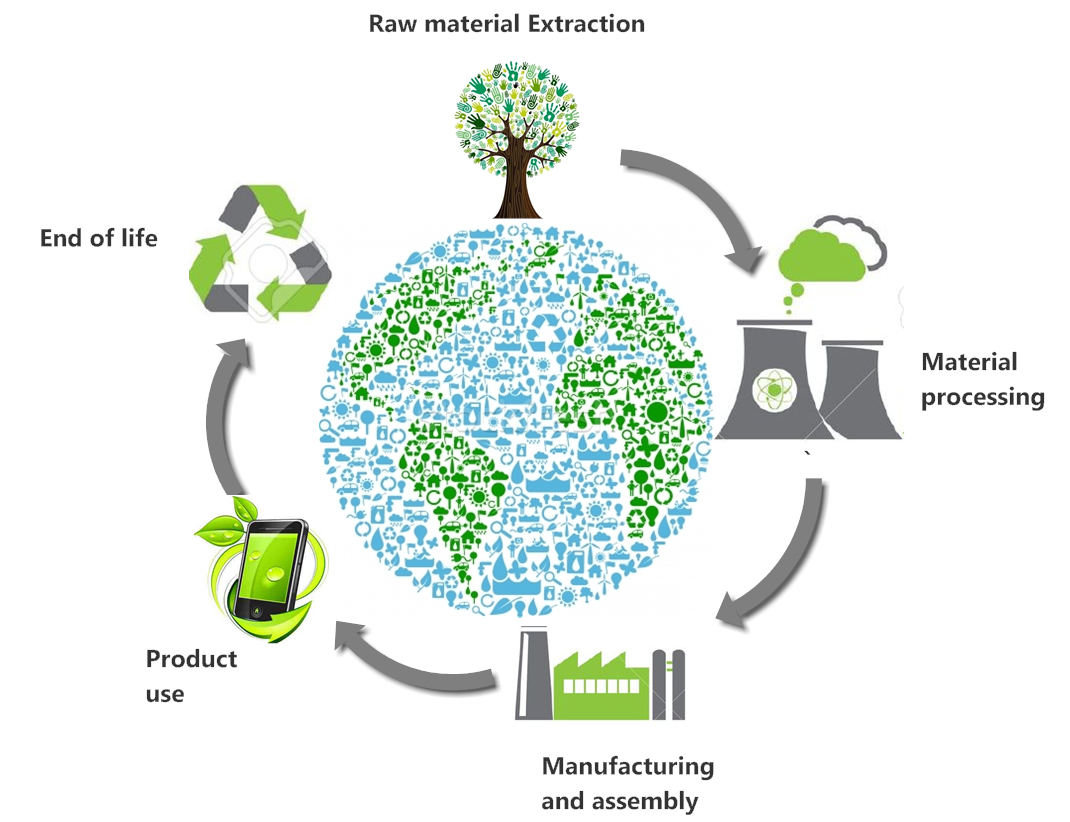
\includegraphics[width=5cm]{cradletograve.png}
	\end{center}\vspace{-5pt}
\caption{LCA variant: Cradle-to-grave.}
	\label{fig:cradleToGrave}
\end{figure} 

\begin{itemize}
\item {\em Goal and scope definition}: This phase defines the focus of the LCA study (product, service or process) along with its granularity and system boundaries. The width and granularity of the system depends on the goal of a particular LCA and includes the functional units, the precise objective being studied or compared and the list of impact categories that are taken into consideration.
\item {\em Inventory analysis}: LCI phase provides with the life cycle inventory, which is an inventory of input/output data with regard to the system being studied and requires data elicitation sufficient for accomplishing the goals of the defined study. The phase takes inventory of incoming flows into the system as an input and flows to across the boundary of the system as an output. Any variant of recourses that are needed to run the system could be served as an input while output can be any type of outcome that is released from system.
\item {\em Impact assessment}: LCIA phase focuses at revealing and assessing the extent and significance of the potential environmental impacts for a product system throughout the life cycle of the product.
\item {\em Interpretation phase}: The last phase provides conclusion and recommendations based on the evaluation and discussions of the results from LCI and/or LCIA.
\end{itemize}

\begin{figure}[!htb]\vspace{-2pt}
	\begin{center}
		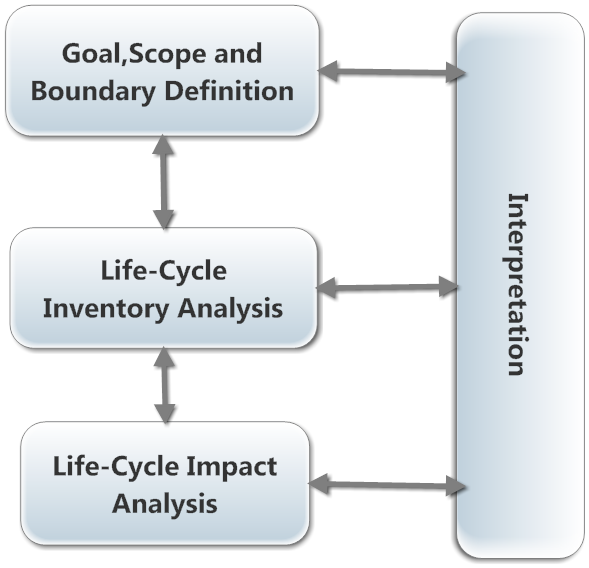
\includegraphics[width=4cm]{LCAproc.png}
	\end{center}\vspace{-5pt}
\caption{LCA framework schematic based on ISO standards.}
	\label{fig:LCA_process}
\end{figure}

\end{comment}


\section{Background and Related Work} 

Among various assessment techniques that fulfill the objective of measuring a product's or a service's environmental impact, ISO LCA\cite{ISO140402006}, Environmental Product Declarations (EPD)\cite{iso2006environmental} and PAS 2050 \cite{pas20082050} tend to be the most acknowledged ones based on the conducted literature review in the scope of this study. Even though EPD provides with an inclusive environmental impact evaluation as well as identifies enhancement prospects, nonetheless, EPD passes over viable problems including carbon storage and the end-of-life phase. Unlike ISO LCA, PAS 2050 standards take into account only a solitary environmental aspect, namely, carbon footprint i.e. total GHG emissions, which makes this technique inflexible and inefficient in terms of identification and assessment of potential trade-offs.
Its reasonable to argue that the comparison of two different products' impacts on the environment in terms of only GHG emissions will be less comprehensive and insightful compared to the holistic environmental impact comparison considering the factors including but not limited to toxic releases, ozone depletion and resource consumption. Whereas, ISO LCA is widely accepted and  possesses capabilities to assess various environmental impacts of products and services \cite{cooper2006life}. Furthermore,  ISO 14000 family, so far, is the unique international standard document on LCA and is referenced by other standardization processes \cite{finkbeiner201340s}. For the rest of this paper the term ISO LCA will be referred as LCA.

Inclusiveness of the LCA method through cradle-to-grave approach and the subsequent circumvention of problem shifting between influences and areas are indicated in \cite{hermann2007assessing} as some of the powerful aspects of LCA methodology. As stated by \cite{guldbrandsson2012opportunities} a number of companies including Ericsson telecom company acknowledges LCA methodology as a worthwhile and suitable framework for evaluating and labeling their products' eco-friendliness. Furthermore, \cite{finnveden2000limitations} compares LCA and Environmental Systems Analysis(ESA) tools in general, and concludes that, LCA is the best option if the objective is to examine the environmental burdens caused by a product or a service.

Although LCA has promising capabilities, it has weaknesses and limitations with its methodological framework as well. Several authors that include but not limited to \cite{joshi1999product, reap2008survey, owens1997life, finnveden1997valuation, arnold1993life, arnold1995environmental, hermann2007assessing} have identified and outlined problems and weaknesses of LCA. As reported by \cite{hermann2007assessing}, LCA being a compound process requires substantial time, effort and data input as well as expert knowledge for its application. In fact, the uncertainty and inaccuracy of the conducted LCA analysis mainly could be due to the input data factors such as quality, quantity, comprehensiveness, oldness  and site specificness \cite{curran2005international, reap2008survey}. In accordance with \cite{joshi1999product} study, when the input at every stage of LCA analysis is limited only to the data associated with major inflows, it will result in immanent boundary definition and comparability problems across systems or products. The steps of LCA methodology as well as its technical and economical strengths have been put into doubt by \cite{finnveden1997valuation, arnold1993life, arnold1995environmental}.

When  it  comes  to  discrete  comparison  of  products  and systems having  unambiguous  and  straightforward  interpretation  or  being distinct  substitutes,  LCA  serves  as  an  efficient tool.  Whereas, according  to  \cite{Bull201410, reap2008survey}, the  trade-off  between more complex and fuzzy products or systems such as between traditional  paper  based  and  corresponding  digital  alternative products, turns out to be a burdensome task for LCA methodology and weakens LCA’s ability to provide accurate environmental  footprint  comparison.  For  the  ICT  sector  specifically, which  is  characterised  by  a  large  number  of  fast  developing, multifunctional  and  multicomponent products,  LCA  analysis faces significant challenges and uncertainties during its phases ascribed to the convolution of the ICT sector, multifunctionality of  ICT  systems, the  intricate  supply  chain  and  the  global market variations, unpredictability of the users attitude towards a  product’s  usage  and  last  but  not  least,  the  data  scarcity, avaliabilness  and  variation \cite{guldbrandsson2012opportunities, Bull201410, farrant2012environmental, enroth2009}. In order to avoid the problem of allocation and multifunctionality of the studied ICT products such as smartphones, laptops, PCs and e-readers, some non-comparative ICT LCA studies allocate or divide the system based on its functionality or based on processes (non-physical division) \cite{choi2006life,frey2006ecological,lu2006balancing, ekvall2001allocation}. 

Analysis of digital products' life cycle have been a subject to a large body of literature. These studies mainly evaluate and quantify ICT products in terms of their environmental impact. The variation in the results of different studies is mainly attributed to the considered system boundary conditions. While doing an LCA case study for electronic mail, \cite{farrant2012environmental} includes ICT equipment manufacturing in the system boundaries and comes to a conclusion that production of ICT equipment is one of the most significant contributors to the environmental impact of the system. Anyhow, the multifunctionality of the ICT equipment in the studied system in \cite{farrant2012environmental} haven't been taken into account. On the other hand, coming to the conclusion that the contribution to the global warming from the electronic teaching aids is from 10 to 30 times higher than the environmental burden posed by printed textbook, \cite{enroth2009} allocates only around 8\% of the environmental impact from the production of ICT equipment to the functional unit of the study. In other words, the latter study takes into account the multi-usage and multifunctionality of ICT equipments used in the system.
Another important aspect is that, the overwhelming majority of conducted LCA studies in this context pay little or no attention to the end-of life management of ICT products. In fact, the end-of life process of electronic products is responsible for 20-50 million metric tons of e-waste per year \cite{koljonen2008environmental}. To further understand the boundary conditions' effect on the final outcome of the LCA study, \cite{gard2002digital} while varying the boundary conditions, conducted a study on printed and electronic scholarly articles. The findings showed that, either printed or electronic scholarly journals were preferable, depending on the assigned boundary conditions.

Surprisingly, while environmental impact of the hardware production, usage and disposal of ICT products such as personal computer (PC), smartphone, e-reader and networking equipment has been broadly considered by a plenty of LCA research studies \cite{guldbrandsson2012opportunities, Bull201410, farrant2012environmental, enroth2009,koljonen2008environmental}, environmental aspects caused by software development attracted only meagre attention of researchers \cite{Moshnyaga:2013}. Indeed, ICT products, in general, do not operate independently without software and heavily rely on softwares such as Operating System (OS) and software applications. The only related work found in the scope of the conducted literature review, using LCA methodology assessed the environmental impact of Linux kernel (an OS)  and K9 Mail (a mobile application) without considering the impact of ICT devices on which the software is executed \cite{moshnyaga2013assessment,Moshnyaga:2013}. The latter study suggests that since software is represented in the so called "cyber or digital world" and the input of raw materials is discarded, the only environmental impacts are originated from the facilities and resources that are in use by developers when documenting and implementing the application. Nowadays vast majority of ICT application, the so called "online applications", which consume energy and resources for continuous syncronization and data transmission over the Internet with their remotely located database servers. However, the author of \cite{Moshnyaga:2013} not being the developer of the K9 Mail application, failed to include its servers in the system boundary scope, henceforth, ignored their contribution to the overall environmental impact of the application.

In LCA studies, especially in ICT LCA, establishment of key issues and obstacles along with avoidance of thorough assessments of inconsequential elements within the life cycle is of superior importance. The screening life cycle analysis of the system's environmental impact with Economic Input Output (EIO) approach, which evolved at Carnegie Mellon University, has been in frequent use by various researchers as an efficient and applicable method for achieving the aforementioned objectives \cite{1208069, junnila2008life, matthews2000extending}. EIO LCA relates the materials and energy resources requirement of the economical activity of the system to the environmental influence resulted from that activity.


\begin{comment}

In fact, according to \cite{cooper2006life}, the survey conducted on LCA practitioners, revealed that the largest portion of the survey participants i.e. 47\% were material production and manufacturers followed by 20\% academia and followed consulting and governmental agencies. Within the context of the type of LCA used, around 77\% of survey respondents analyzed products using LCA studies based on IS0 14040 standards and 69\% used EIO LCA method. Out of all respondents 54\% use both, hence leaving 15\% of respondents never using ISO LCA and 23\% of respondents never using EIO LCA methods.

\end{comment}

\section{Business Card Systems}

Prior to the widespread expansion of ICT products and Internet, the only existing manner of exchanging business cards was through manual interchange of traditional printed business cards (PBC). Despite the nowadays popularity of ICT technologies, PBC are still intensively used for commercial as well as personal purposes. In the PBC system which is shown in Figure \ref{PBCSystem}, customers manually exchange printed business cards, which are obtained during a lengthy process, which includes extraction and processing of raw materials, manufacturing of paper, printing, transportation, usage and end-of-life treatment. While in the DBC system, which is represented in Figure \ref{DBCSystem}, customers exchange business cards in a digital format over the Internet using a DBC software.

\begin{figure}[h]
\centering
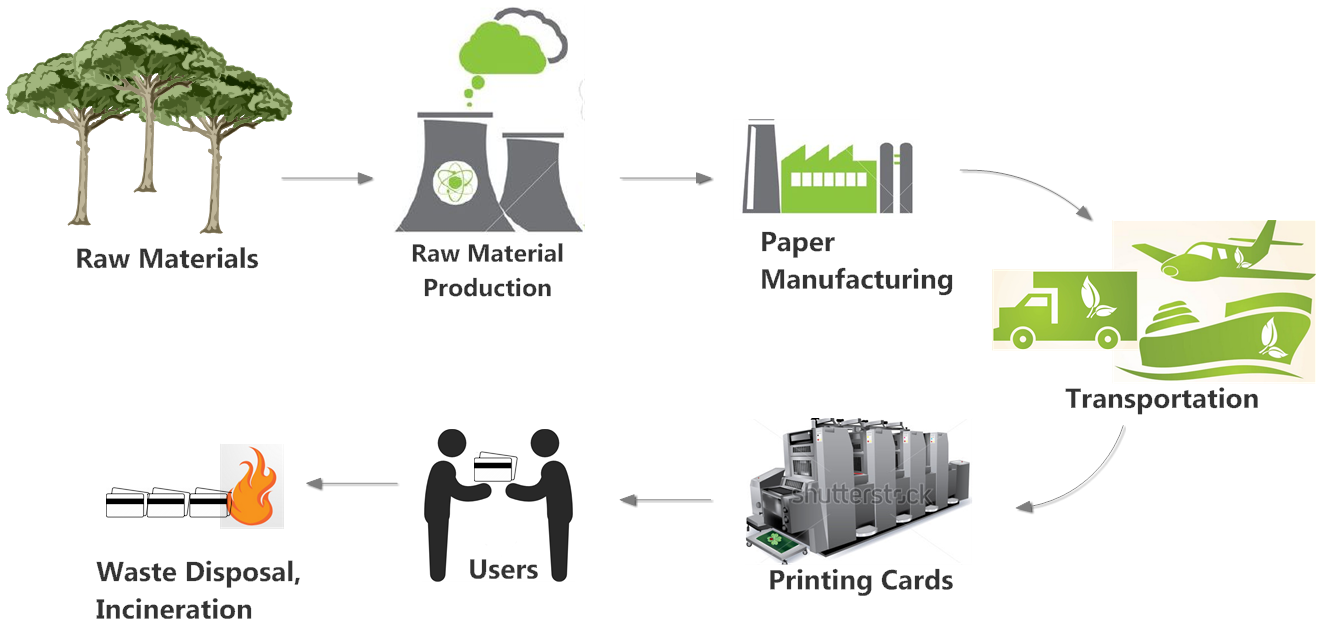
\includegraphics[width=6cm]{PBCSystem1.png}
\caption{PBC System}
\label{PBCSystem}
\end{figure}

\begin{figure}[h]
\centering
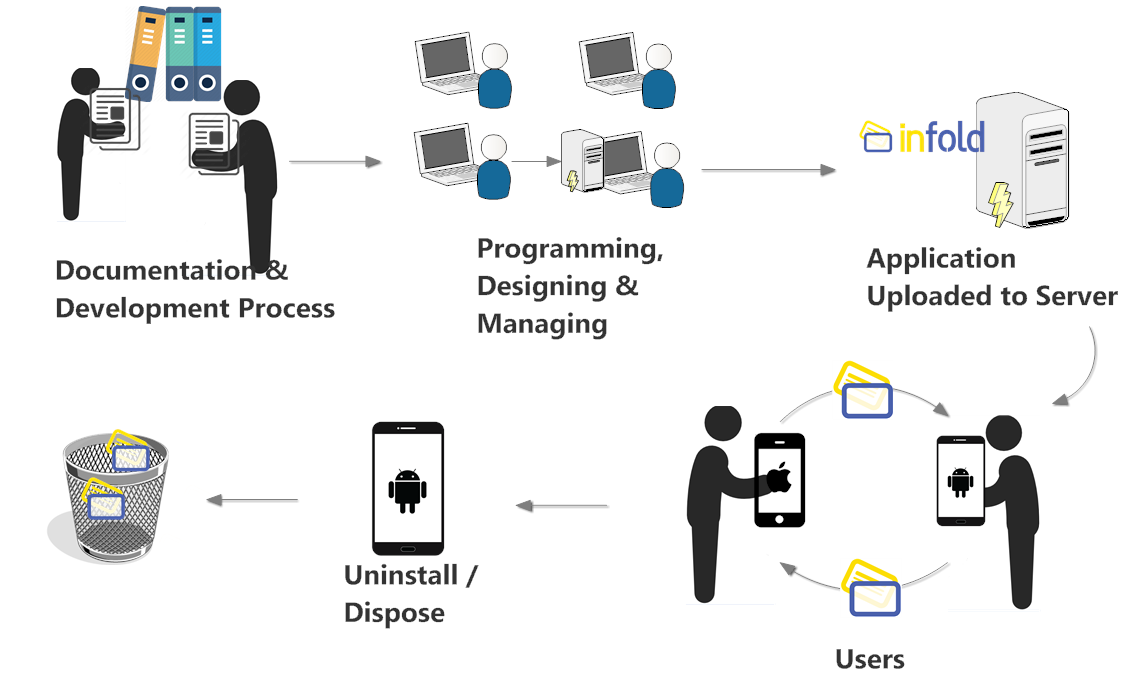
\includegraphics[width=6cm]{DBCSystem.png}
\caption{DBC System}
\label{DBCSystem}
\end{figure}
The DBC software refers to a mobile application that facilitates the exchange of information packets between two or more customers through an Internet infrastructure including database servers and smartphones. Although, there exists a variety of DBC software including but not limited to Card Flick, CamCard, Snapdat, One Card, Flextown, none of them fulfills the purpose and assumptions made in this study. In the scope of this research as a DBC software was chosen mobile application Infold, more specifically its version 0.1, which were developed specifically for the purposes of this study. Unlike the aforementioned alternatives, it supports only a single functionality, which is the creation and exchange of digital business cards and satisfies all the assumptions considered in this paper. The more detailed explanation of DBC and PBC systems is covered in subsections \ref{DBCBoundary} and \ref{PBCBoundary}.

\section{Method}

Life cycles of the two studied systems in this paper have been separately modeled in accordance with IS0 14040 LCA methodology. A two-stage cradle-to-grave life cycle analysis has been applied to PBC and DBC systems for identifying and evaluating life cycle impact categories as well as  total energy consumption, GHG emissions and toxic releases. The first stage (screening analysis) relies on the EIO approach that is capable of determining the principal sectors requiring more thorough analysis as well as providing a general evaluation of energy demand and environmental burdens associated with the studied systems. The second stage is based on the ISO LCA methodology and aims at providing a comprehensive examination and quantification of life cycle impact categories and burdens considering the findings from the first stage. 

\begin{comment}

\begin{table}[htbp]
\caption{Life Cycle Model Elements: PBC System}
\begin{center}
\begin{tabular}{|l|l|}
\hline
\textbf{Material Production} & Ink Production, Paper Production \\ \hline
\textbf{Manufacturing} & Paper Manufacturing \\ \hline
\textbf{Distribution} & Paper delivery \\ \hline
\textbf{Printing} & Card Sizing, Collection and Storage, Personal Transportation  \\ \hline
\textbf{Use} & Card Exchange \\ \hline
\textbf{End-of-Life} & Card Disposition, Card Recycling \\ \hline
\end{tabular}
\end{center}
\label{PBCTable}
\end{table}


\begin{table}[htbp]
\caption{Life Cycle Model Elements: DBC Card System}
\begin{center}
\begin{tabular}{|l|l|}
\hline
\textbf{Material Production} & None \\ \hline
\textbf{Manufacturing} & Software Development Process, Facilities used by developers \\ \hline
\textbf{Distribution} & Downloading the application \\ \hline
\textbf{Use} & Registering, Exchanging cards \\ \hline
\textbf{End-of-Life} & Uninstalling the application \\ \hline
\end{tabular}
\end{center}
\label{DBCTable}
\end{table}

\end{comment}

\begin{comment}

\subsection{Goal Definition and Scope }

The paper is comparing two different products, namely DBC and PBC, that fulfill the same functionality, which is an exchange of business cards between two or more customers. The comparison is based on life cycle approaches for resource and energy consumption and environmental aspects of PBC and DBC systems. The findings of this study could be used for marketing and regulating the use of DBC and PBC without aiming at identifying the possible improvements for them.\\

\end{comment}


\subsection{General Assumptions}\label{Generalassume}
To compare DBC and PBC systems, some general assumptions were required which apply to both stages of this LCA analysis and are detailed below.

\begin{itemize}
\item The customer in this paper is identified as a person who possesses a PBC or uses the DBC software for creating and exchanging business cards.
\item Assuming that each company prints business cards annually, the lifetime considered for exhausting all business cards is one year.
\item PBC system scope is only a single functionality, that is the exchange of business cards, whereas DBC software could have multiple functionality  including but not limited to exchange, management, broadcast, copy and translation of business cards. For simplicity and equivalent comparison between DBC and PBC systems, other functionality of these systems are not taken into consideration. This makes the complexity of allocation and multifunctionalilty of DBC system to be easily avoided.
\item The utilized energy during operation of the DBC software was measured using powerTutor mobile application (approximately 0.002778 Wh/exchange). The powerTutor was built by Google Inc. in collaboration with University of Michigan \cite{zhang2010accurate}. In fact, the measured energy usage is an upper bound.
\begin{comment}
The considered DBC software is free of any advertisements add-ons, henceforth is sustainable because most of the smartphone energy is consumed for locating the customer and providing him/her with addons. This is covered in \cite{pathak2012energy} and the study shows that 25 to 35 percent of energy consumption is by application functionality and the remaining is due to addons.
\end{comment}
 \item Since each DBC has an average size of 10 KB, then each one to one exchange between two customers is an exchange of 40 KB data over the Internet which includes the information packet header's size. From \cite{Moshnyaga:2013}, its assumed that 1 MB of traffic across the Internet takes 5.9 Wh which includes cooling, UPS, wiring, broadband routers, telephone lines. From \cite{EnergyDownload}, its assumed that the server and networking equipment consume 2.6 Wh/MB, cooling and losses contribute additional 1.3 Wh/MB, embedded infrastructure energy uses 0.9 Wh/MB and the DSL Access Multiplexers (DSLAMs) and phone line require 1.1 Wh/MB. Therefore, the overall required energy consumption for each one to one exchange is up to 5.9 Wh/MB,  which is an upper bound.
\item The energy consumption from the DBC software update has not been considered because the functionality of the product is already fulfilled and there is no need for the customer to update his/her software.
\item The dedicated effort and cost for the development of the future updates of the DBC software is not taken into account.
\item The environmental impact from the production of server used in DBC system is considered since it is allocated specifically for the purposes of DBC software.
\item Servers usually have more than one year lifetime, however, the considered production cost of server used in the DBC system is for one year.
 \item An upper-bound energy consumption of server used in the DBC system was estimated to be 45 Wh based on the data from the hosting provider (Digital Ocean).
\item For simplicity and fair impact assessment the environmental impact originated from the production and manufacturing of a smartphone used in DBC system has not been taken into account, since it is not utilized specifically for the DBC software and should be amortized over the active smarthphone applications which significantly varies among customers.
\item Due to a highly complex structure and diverse functionality of the Internet, this paper ignores all the environmental impacts and energy depletion associated with the components and devices in the Internet except the ones that directly relate to an exchange of DBC over the Internet.
\end{itemize}

\begin{comment}
Table \ref{AppTable} and Figure \ref{apps2013} include information regarding the average number of active applications in smartphones for various countries. The latter information was obtained from The Our Mobile Planet online tool. The Our Mobile Planet research was originated by Google and performed by Ipsos MediaCT. \cite{Flurry} conducted a study on smartphone applications usage other than calling, SMS, MMS, video calling and camera usage of average american mobile user. Accroding to \cite{Flurry}, out of total application usage 32\% were games, second highest was Facebook application having 18\%. Currently more than 1 million applications exist in Google Play and Apple Store, hence it is quite difficult to amortize the smartphone production cost over the applications.

According to statistics published in "The US mobile App report" by ComScore\footnote{ComScore is a leading Internet technology company that conducts statistical Analytics for cyber world} among average American citizens older than 18 years old  Facebook application ranked the top popularity with 72.6\% followed by Youtube application and Google Play with 52.6\% and 45.6\% respectively. Observations from the latter two statistics conclude that dividing the production cost of a smartphone with 26 applications including but not limited to SMS, MMS, camera usage and video calling will not lead to fair impact assessment for the DBC sytem considered in this paper. Nonetheless, for the completeness of this study calculations and analysis were performed evaluating environmental impacts of DBC system including and excluding the production cost of the smartphone.


\end{comment}

\subsection{Functional Unit}\label{sec:FunctionalUnit}

A functional unit defines the foundation of LCA for comparing two or more products. All the data collected in the inventory will be dependent on the defined functional unit.
\begin{comment}
For example, in the comparison of plastic and paper bags, the functional unit will be the volume of groceries carried by each bag option. If, for instance, one plastic bag carries twice the volume of groceries than a paper bag, then these products cannot be compared on a one to one basis since they are not containing the same amount of grocery. In this scenario, two paper bags will be determined as having an equivalent function of one plastic bag. However,
\end{comment}
In this study, DBC and PBC products are compared on a one to one basis. An exchange of each of them between two customers requires an exchange of two business cards or two equivalent information packets. 
\begin{comment}
In general, an exchange amongst $n$ customers requires $n(n-1)$ paper based business cards or $n(n-1)$ information packets.
Most printing services produce a minimum of 50 cards per user and we need two users to exchange business cards with each other. A more realistic scenario would be 50 users printing 50 cards each and exchanging $50 * 49$ times.
\end{comment}
It is worth mentioning that in DBC system, a customer can broadcast a single information packet representing the business card to other customers which is much more efficient in terms of bandwidth consumption rather than a one to one exchange. Even though the latter functionality is energy beneficial to DBC system, but for the unbiased comparison, it is not considered since there is no feasible way to broadcast in PBC system.

In order to obtain a comprehensive and accurate picture of DBC and PBC system's life cycle impacts, a flexible functional unit has been chosen for this study. More precisely, two cases of functional units were considered; a case of 1000 exchanges between customers in PBC and DBC systems, that is production and exchange of 2000 PBC and DBC respectively and a case of 33000 exchanges between customers in PBC and DBC systems or production and exchange of 66000 PBC and DBC respectively. The latter case is a real world scenario based on the data and statistics regarding annually utilized business cards provided by the Human Resource department at Masdar Institute of Science and Technology.  


\subsection{PBC System Boundary} \label{PBCBoundary}
Life cycle model of the PBC system is composed of five major stages which along with their model elements are listed in Table \ref{PBCboundary}. A brief description of each stage and corresponding model elements is provided below.

A PBC, generally, is composed of paper and ink. These components are acquired from chemical manufacturing and paper manufacturing processes which require natural resources. Paper manufacturing sector is not available in some countries, hence the transportation of paper based products could be included in the according stage. After obtaining the paper with a suitable quality, thickness and predetermined size, PBC design procedure begins followed by the printing stage. Hereafter, already made PBC are collected and stored in the appropriate facilities and then delivered to the customers. Then costumers exchange PBC during various events including conferences and meetings. When the useful life of the PBC is expired, the product is disposed as a municipality waste or incinerated.   

\begin{comment}
\begin{itemize}
\item {\em Material Production}; In general, paper based cards are composed of paper and ink, which are  acquired from natural resources available in abundance and chemical manufacturing processes respectively. 
\item {\em Manufacturing}; Paper based products manufacturing have pre-defined standards such as the weight, thickness, filling and quality of the paper.
\item {\em Distribution};Paper manufacturing sector is not available in some countries, hence the transportation of paper based products are also considered as part of the PBC system's life cycle.
\item {\em Printing}; Storage and transportation costs of printed PBC are included in the life cycle of PBC system.
\item {\em Use}; A customer already possessing PBC will exchange them with other customers.
\item {\em End-of-life}; In the end-of-life stage of PBC system's life cycle, most of the PBC are disposed as a municipality waste or incinerated.
  
\end{itemize}

\end{comment}

\begin{table}[h]
\caption{Life Cycle Model of the PBC System}
\centering
\begin{tabular}{|l|l|}
\hline
\textbf{Life Cycle Stage} & \textbf{Model Elements}           \\ \hline
Material Production       & Paper Production, Ink Production \\ \hline
Manufacturing             & PBC Creation and Printing        \\ \hline
Distribution              & Facility Infrastructure, Collection \\
& and Storage, PBC Delivery \\ \hline
Use                       & PBC Exchange                     \\ \hline
End-of-Life               & PBC Disposal                     \\ \hline
\end{tabular}
\label{PBCboundary}
\end{table}




\subsection{DBC System Boundary}\label{DBCBoundary}

DBC system boundary is quite different from the system boundaries of traditional industrial products. The life cycle model of the DBC system considered in this paper is similar to the one in \cite{Moshnyaga:2013, moshnyaga2013assessment} and along with the model elements is detailed in Table \ref{DBCboundary}. A brief description of each stage and corresponding model elements is provided below.

The DBC system has no raw materials as an input to the system. The manufacturing stage of the DBC system involves typical software engineering process, as well as tools and facilities used by the corresponding personnel in charge of the development of the DBC software. The aforementioned facilities and tools include but are not limited to custom softwares like Eclipse IDE, Android Studio and equipments like PCs, Air Conditioner, UPS, printer, and lighting. After the manufacturing stage, the DBC software is deployed online so that it is accessible for customers. Once the DBC software is downloaded and installed on a smartphone, a customer starts using the software for creating and exchanging DBC, during which the according information packets are routed through the Internet. Further environmental burdens are associated with the production and disposition of the server. Finally, end-of-life stage is simply uninstalling the DBC software from a smartphone. 

\begin{comment}
\begin{itemize}
\item {\em Manufacturing}; Typical software engineering development process including requirements engineering, object oriented design, validation and testing. Actual development and coding of the DBC software. Facilities used by developers to develop the application.
\item {\em Distribution}; Downloading the application from server to phone is similar to distribution of tangible products such as phone or PC.
\item {\em Use}; Usage of the application which includes exchange of business cards between customers. 
\item {\em End-of-life}; End-of-life of the application is simply uninstalling the application from smartphone.
\end{itemize}
\end{comment}

\begin{table}[h]
\caption{Life Cycle Model of the DBC System}
\centering
\begin{tabular}{|l|l|}
\hline
\textbf{Life Cycle Stage} & \textbf{Model Elements}                                                                                                                                                            \\ \hline
Manufacturing             & \begin{tabular}[c]{@{}l@{}}Software Engineering, DBC Software Development, \\ Facility Infrastructure\end{tabular}                                                                \\ \hline
Distribution              & DBC Software Installation                                                                                                                                                         \\ \hline
Use                       & \begin{tabular}[c]{@{}l@{}}Server Production and Disposal, Smartphone Use, \\ File Transfer, DBC Creation and Exchange\end{tabular} \\ \hline
End-of-Life               & DBC Software Uninstallation                                                                                                                                                       \\ \hline
\end{tabular}
\label{DBCboundary}
\end{table}


\begin{comment}


\begin{figure}[h]
\centering
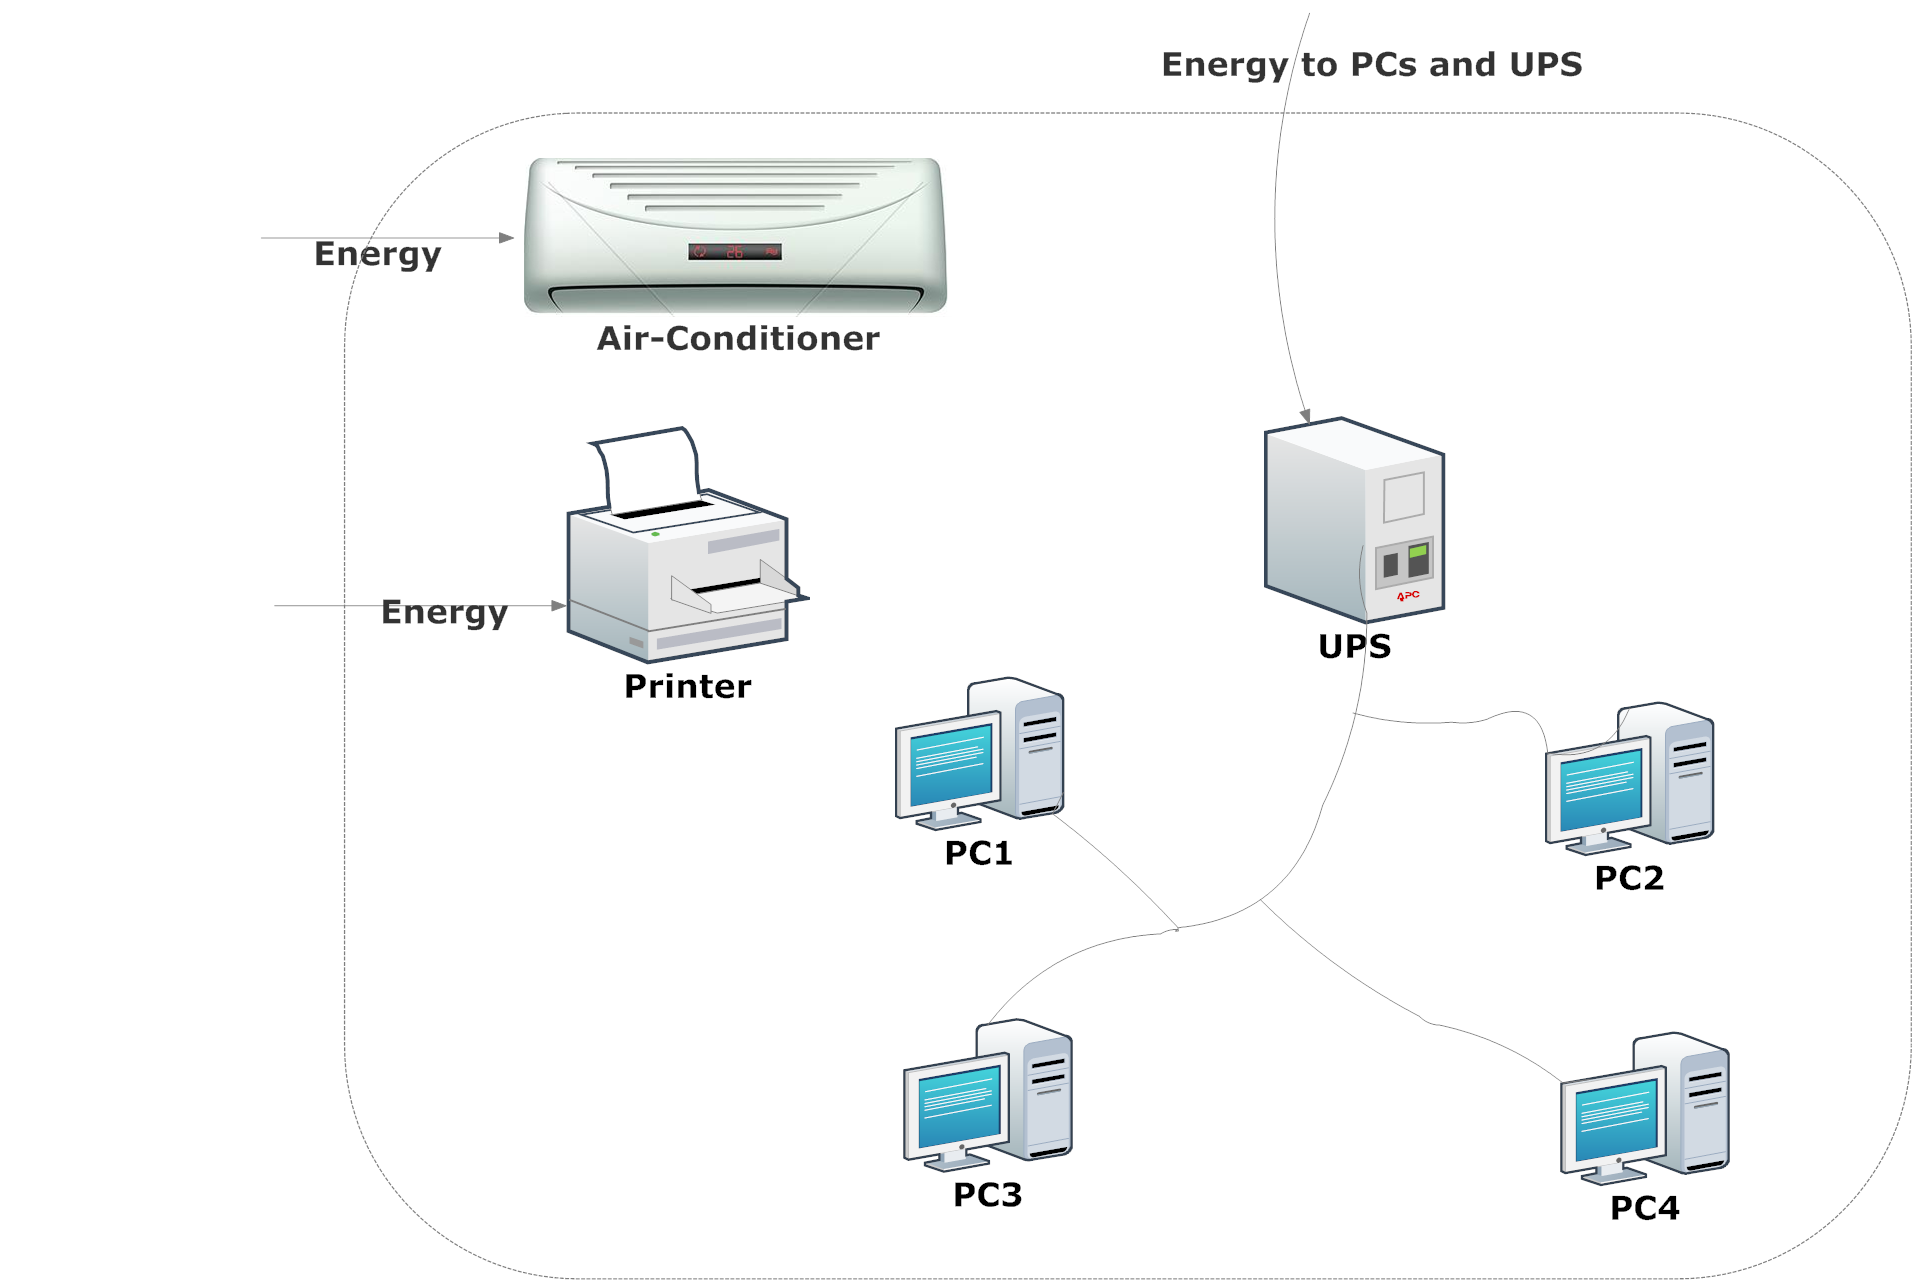
\includegraphics[width=8cm]{comprehencsiveLAST.png}
\caption{System boundary of the production phase of DBC software}
\label{fig:ICTboundary}
\end{figure}

\begin{figure}[h]
\centering
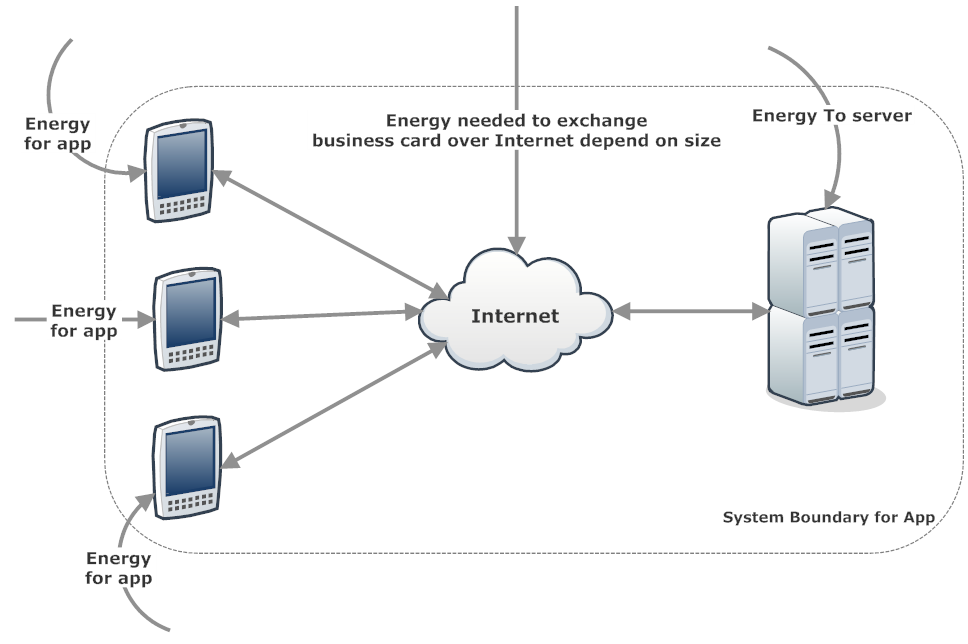
\includegraphics[width=8cm]{systemboundryICT.png}
\caption{DBC software during use phase}
\label{figDBCuse}
\end{figure}


\end{comment}


\section{Screening Analysis} \label{ScreeningLCA}

\begin{comment}
The EIO LCA method is practical for conducting a screening analysis of the environmental impacts of a complex systems like ICT products or services. 
\end{comment}
As a first stage of this LCA study a screening of the environmental impacts and energy consumption has been carried out by applying EIO LCA methodology to PBC and DBC systems. The analysis was performed using Carnegie Mellon EIO LCA online tool, which uses U.S. data from 2002 \cite{Mellon}. The monetary expenses were calculated for DBC and PBC systems in both cases of functional units and served as an input to EIO LCA. The calculations for the DBC system are shown in Table \ref{PBCcalc}. For the PBC system's calculations it was assumed that the average cost of printing 200 standard business cards is 50 USD. This assumption was based on the extensive observations on the price statistics offered by various U.S. based business card printing services.


\begin{table}[htbp]
\caption{Monetary Expenses of the DBC system}
\begin{center}
\begin{tabular}{|l|l|}
\hline
\textbf{Production of a server} & 240 USD annually \\ \hline
\textbf{Production of a software} & 8000 USD \\ %\hline
(all inclusive cost considering &  \\
expenses associated with &  \\ 
the corresponding personnel & \\
and facilities) & \\\hline
\textbf{Server energy consumption} & 45 Wh hence,\\ %\hline
 & 394.2 KWh annually \\ \hline
\textbf{Energy consumption from software installation} & 236 Wh\\ (for 1000 exchanges) & \\ \hline
\textbf{Smarpthone energy consumption} & 2.778 Wh \\ 
(for 1000 exchanges) & \\ \hline
\textbf{Total energy and monetary expenses} & 394.439 KWh\\
 (software installation + smartphone + server) & given the average \\
 for the case of 1000 exchanges & global price of electricity\\
 & 0.5 USD per KWh,\\
& total expenses are \\
& 197.22 USD \\
\hline

\textbf{Total energy and monetary expenses} & 406.1389kWh,   \\ 
for the case of 33000 exchanges & hence total\\
& expenses are \\
& 203.06945 USD \\
 \hline
 

\end{tabular}
\end{center}
\label{PBCcalc}
\end{table}


 \subsection{Results}
Results of a first screening of the environmental impacts and energy consumption of PBC and DBC systems for both cases of functional units i.e. 1000 and 33000 exchanges are presented in Figure \ref{screen1} and Figure \ref{screecn3Sectors}. The toxic releases shown in Figure \ref{screen1} refer to different environments such as surface and under water, land, air and include metals and non metals. For the case of 1000 exchanges Figure \ref{screen1} shows that the PBC system has less environmental impact, energy consumption and toxic releases compared to the DBC system. On the contrary, the lower graph in Figure \ref{screen1} clearly shows that for the case of 33000 exchanges the DBC system is far more environmentally friendly than the PBC system emitting almost 6 times less amount of GHGs than the PBC system. Likewise, the PBC system's consumed energy and toxic releases are nearly 9 and 15 times higher than those of the DBC system respectively. The results shown in Figure \ref{screecn3Sectors} indicate that energy consumption of the PBC system is mainly driven by three major sectors, namely, paper mills, power generation and supply and printing, which account for 31\%, 26\% and 10\% of the total energy demand respectively. Moreover, it could be inferred, that compared to energy usage of the DBC system, where the crucial energy consuming sector is power generation and supply, which demands 75\% of the cumulative energy consumption, energy usage of the PBC system is more evenly distributed between sectors. 

The aforementioned results can be explained by the fact that cost of the development of the DBC software and the production of server used in the DBC system is not amortized over large number of exchanges. The considered server as well as the DBC software can easily handle thousands of customers. It is safe to assume that the higher the number of exchanges the more amortized is the cost. More importantly, PBC system does not take into account any printing and manufacturing machinery production cost which is making the PBC system ranked better than the DBC system in terms of environmental impact and energy demand.

\begin{comment}
In a real world scenario, the number of business cards printed annually by a medium size company are significantly higher than 1000. In fact, according to Masdar Institute's Human Resource department, about  66000 business cards are printed annually. Since printing 66000 PBC requires more energy, it produces more toxic releases to the atmosphere than 66000 DBC.

Gas pollutants shown in Figure \ref{screen2} refer to common released gases from the industry including but not limited to nitrogen oxide, sulphur oxide and carbon monoxide. As could be seen from Figure \ref{screen2} in the case of 1000 exchanges  carbon monoxide emissions from DBC system are 3 times higher than from PBC system. On the contrary, carbon monoxide emissions from PBC system are about 20 times higher compared to carbon monoxide emissions of DBC system in the case of 50000 exchanges. The similar tendency could be observed for the other gas pollutants.
\end{comment}

\begin{figure}[h]
\centering
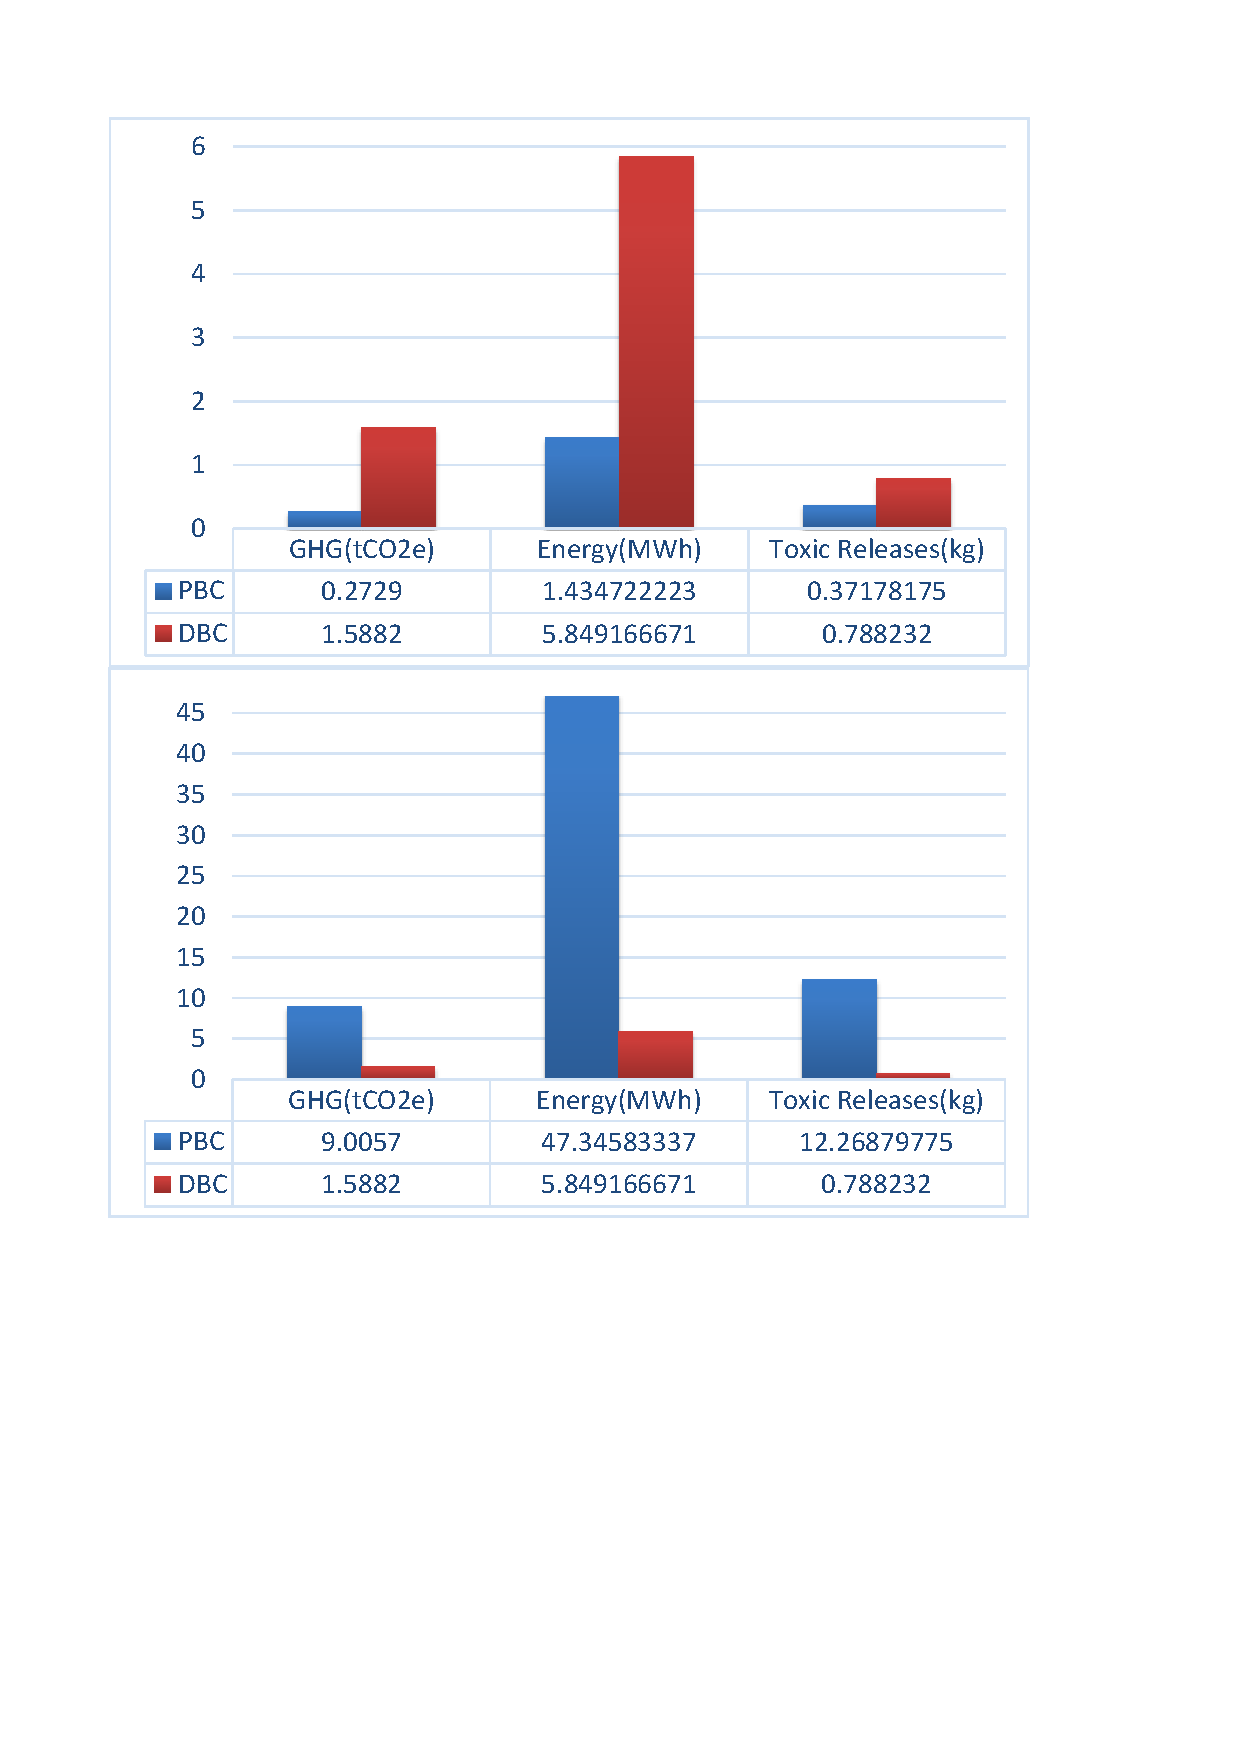
\includegraphics[width=6cm]{EIO-LCA.pdf}
\caption{Environmental impacts of PBC and DBC systems for 1000 and 33000 exchanges of business cards on top and bottom respectively}
\label{screen1}
\end{figure}

\begin{comment}
\begin{figure}[h]
\centering
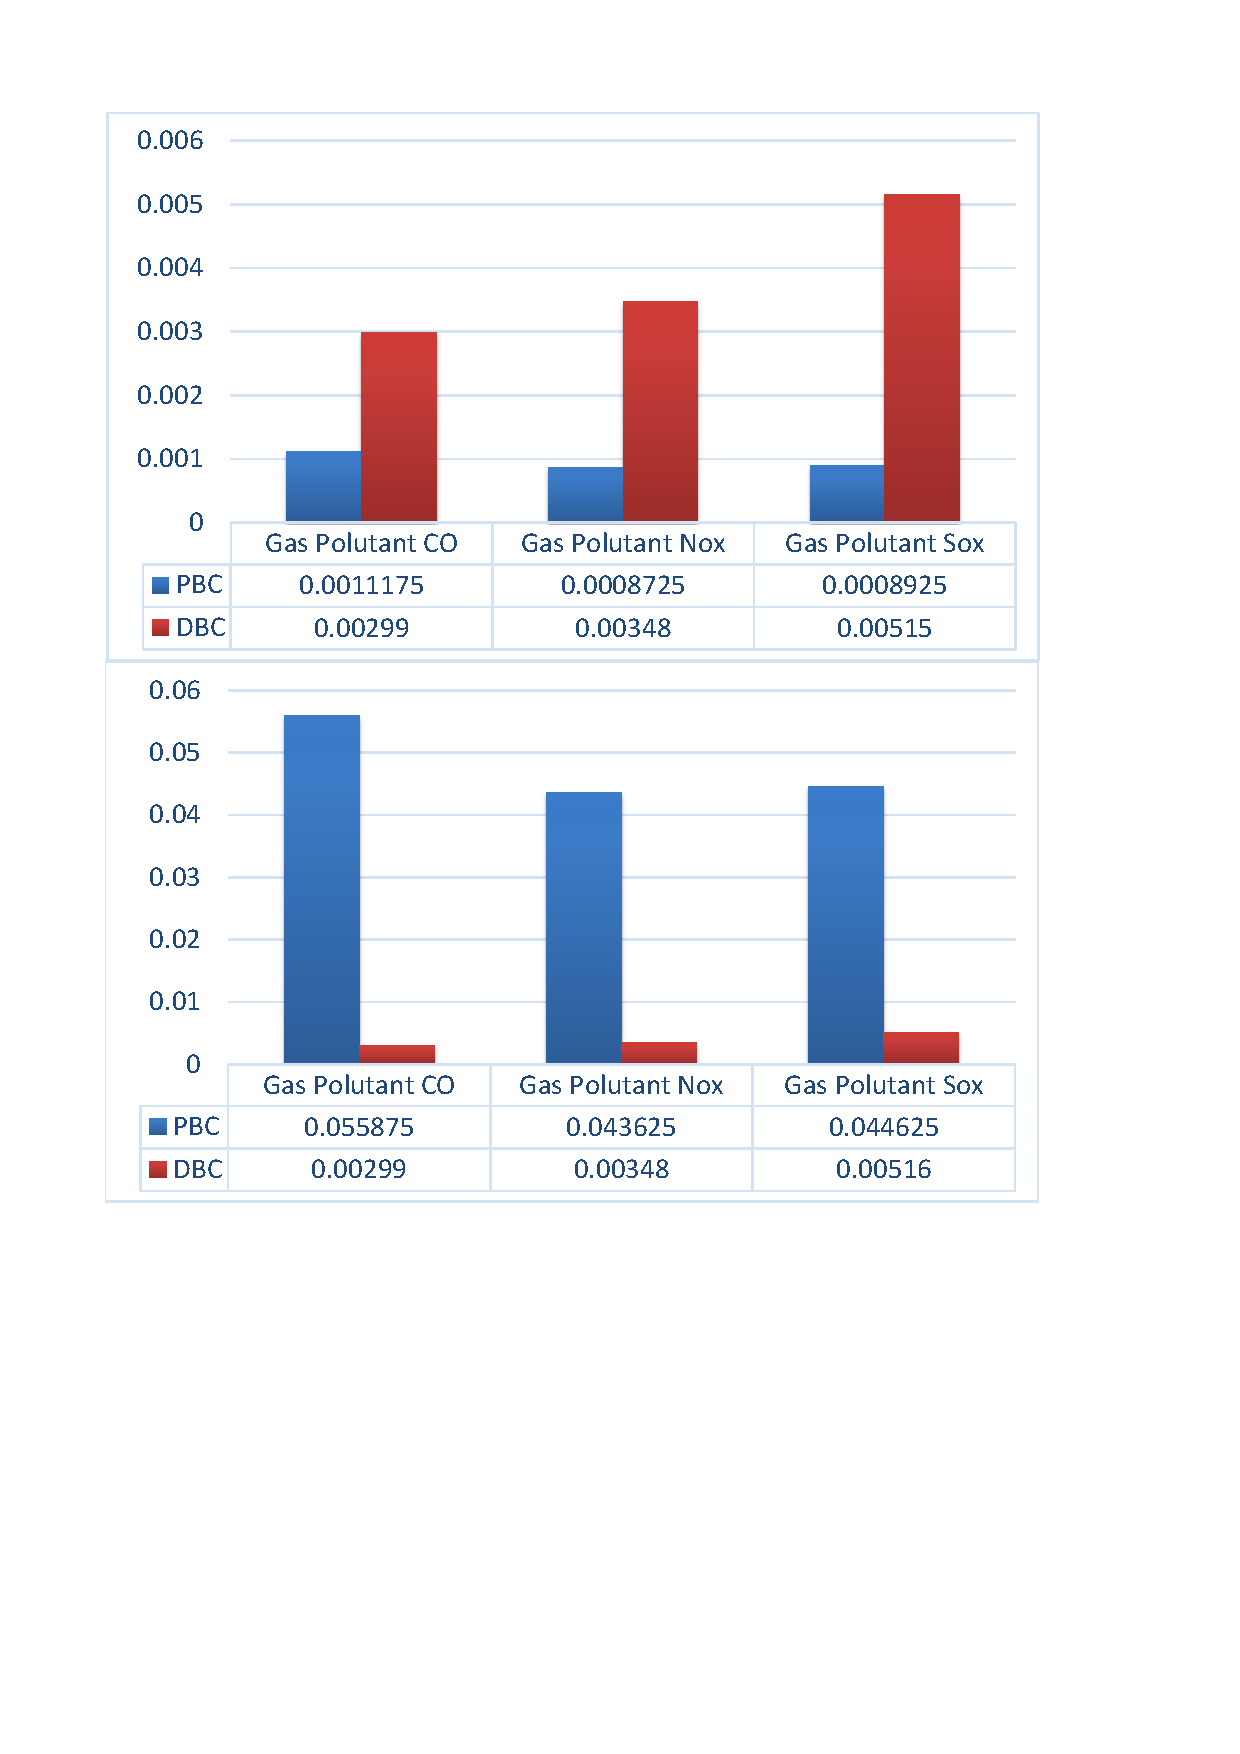
\includegraphics[width=6cm]{screen2.pdf}
\caption{Gas pollutants released by PBC and DBC systems for 1000 and 50000 exchanges of business cards on top and bottom respectively}
\label{screen2}
\end{figure}
\end{comment}


\begin{figure}[h]
\centering
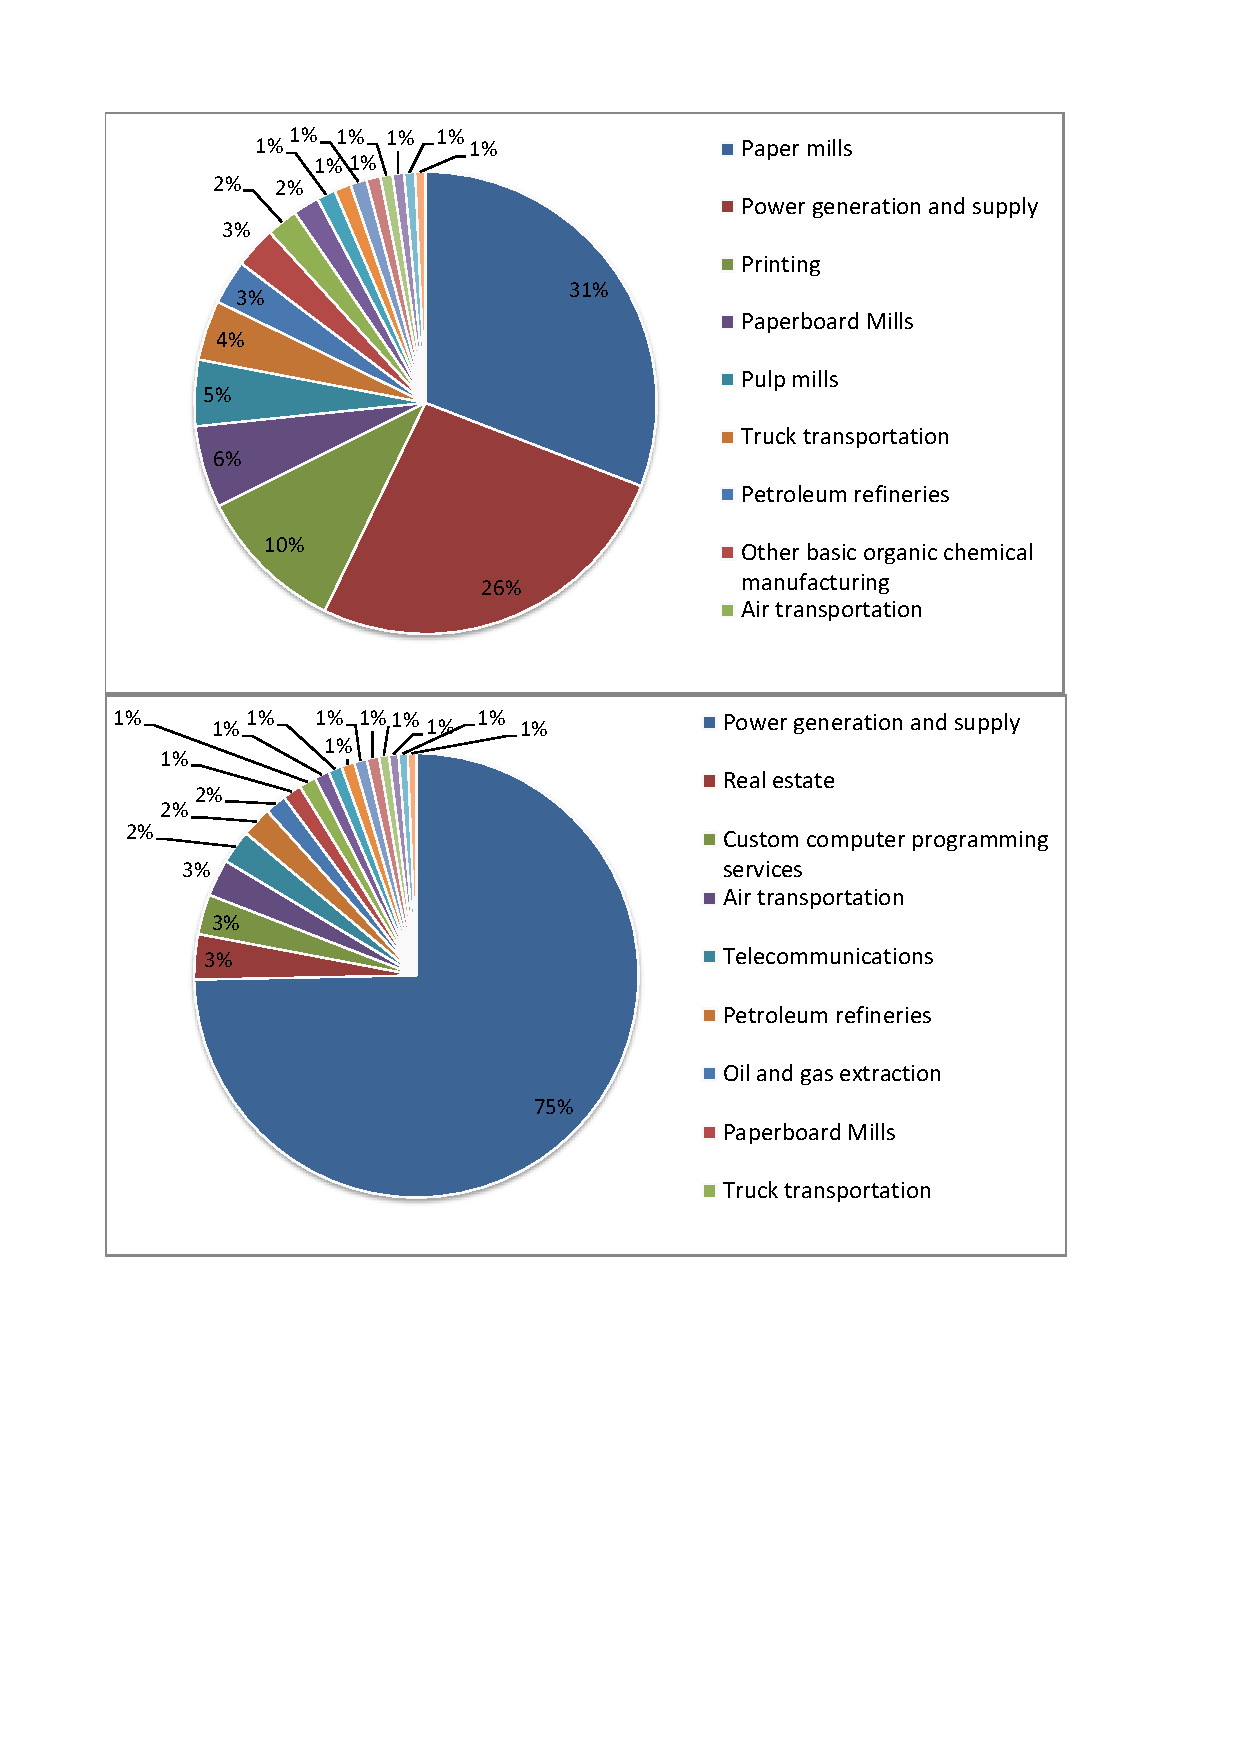
\includegraphics[width=6cm]{screen3.pdf}
\caption{Energy contribution percentage of each sector to the cumulative energy demand of DBC and PBC systems on bottom and top respectively}
\label{screecn3Sectors}
\end{figure}

\section{Second Stage Analysis}
Based on the intensive literature review, it has been found that SimaPro software is one of the most used life cycle assessment applications, which was the reason for using it for the purpose of this study. Ecoinvent 3.1 databases of the SimaPro software were used as an inventory database for both PBC and DBC systems.

\subsection{Life Cycle Inventory}
Data collection and calculations performed in the Life Cycle Inventory (LCI) phase of this LCA analysis, which quantify associated inputs and outputs in the PBC and DBC systems are detailed below as well as provided previously in subsection \ref{Generalassume}. 

Dimensions of the standard PBC were considered to be 3.37 inches in width and 2.125 inches in height based on ISO/IEC 7810 Identification cards' standard.  The standard quality business card paper weight was considered to be 350 g per $m^2$. Considering the latter two facts, the weight of one PBC was estimated to 1.63824 g. When printing PBC some space of paper is left empty to avoid overlapping between cards. This is usually referred as bleed space which is 0.125 of the height and width of PBC. Hence the weight of a single PBC has been considered to be 1.8194 g. The server used in the DBC system for facilitating exchanges has the following specifications; Intel(R) Xeon(R) CPU E5-2630L v2 @ 2.40GHz, 1GB Ram, 30GB SSD Hard Disk. Smartphones used for exchanging DBC were Samsung Galaxy S4 and LG Nexus 4.

The results of the second stage of this LCA study are shown in Figure \ref{fig:onescore} and Table \ref{PBCandDBCexchanges}. These results represent a single score comparison between both systems in terms of Ecopoints\footnote{Ecopoints are a composite measure of the overall environmental impact of any material, product or service}. One can easily notice from the results that the life cycle impacts of the PBC system heavily depend on the number of exchanges. In fact, the impacts increase linearly with the number of exchanges. Also, it could be observed that DBC system's impacts mainly depend on the fixed cost which is nothing else but the development cost of the DBC software and the manufacturing cost of server hardware. 

When comparing the PBC and DBC systems with variable functional units, impacts depending on the exchange procedure in the DBC system are significantly less compared to PBC system.  

This finding is in confirmation with our previous findings of screening analysis using EIO LCA approach. However, as expected, there were significant numerical differences between the results of full LCA and screening analysis. More specifically, the case of 1000 exchanges, the screening analysis revealed a considerable difference between the environmental impact and energy consumption of DBC and PBC systems in favor of PBC, which were estimated to be about 4 times. Nonetheless, the results of full LCA analysis indicated that the environmental impact of PBC and DBC systems in the case of 1000 exchanges varies only by a small amount. Moreover, for the case of 50000 exchanges, the difference between full LCA and EIO LCA is even more solid.

\begin{figure}[h]
\centering
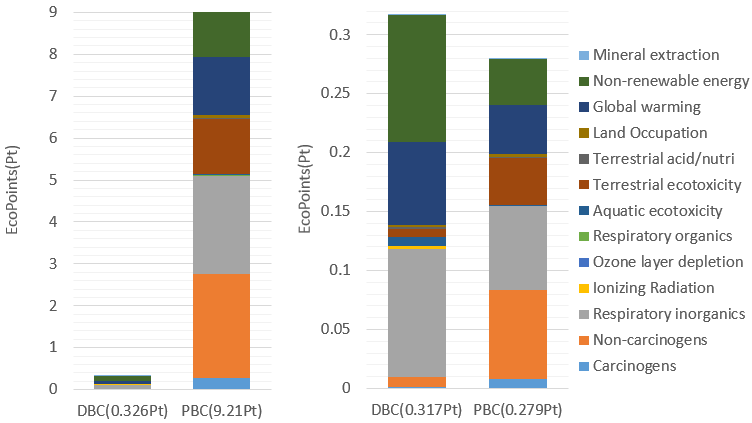
\includegraphics[width=9cm]{lasttt.PNG}
\caption{Environmental impacts of PBC and DBC systems for 1000 exchanges in terms of Ecopoints}
\label{fig:onescore}
\end{figure}

\begin{comment}

\begin{figure}[h]
\centering
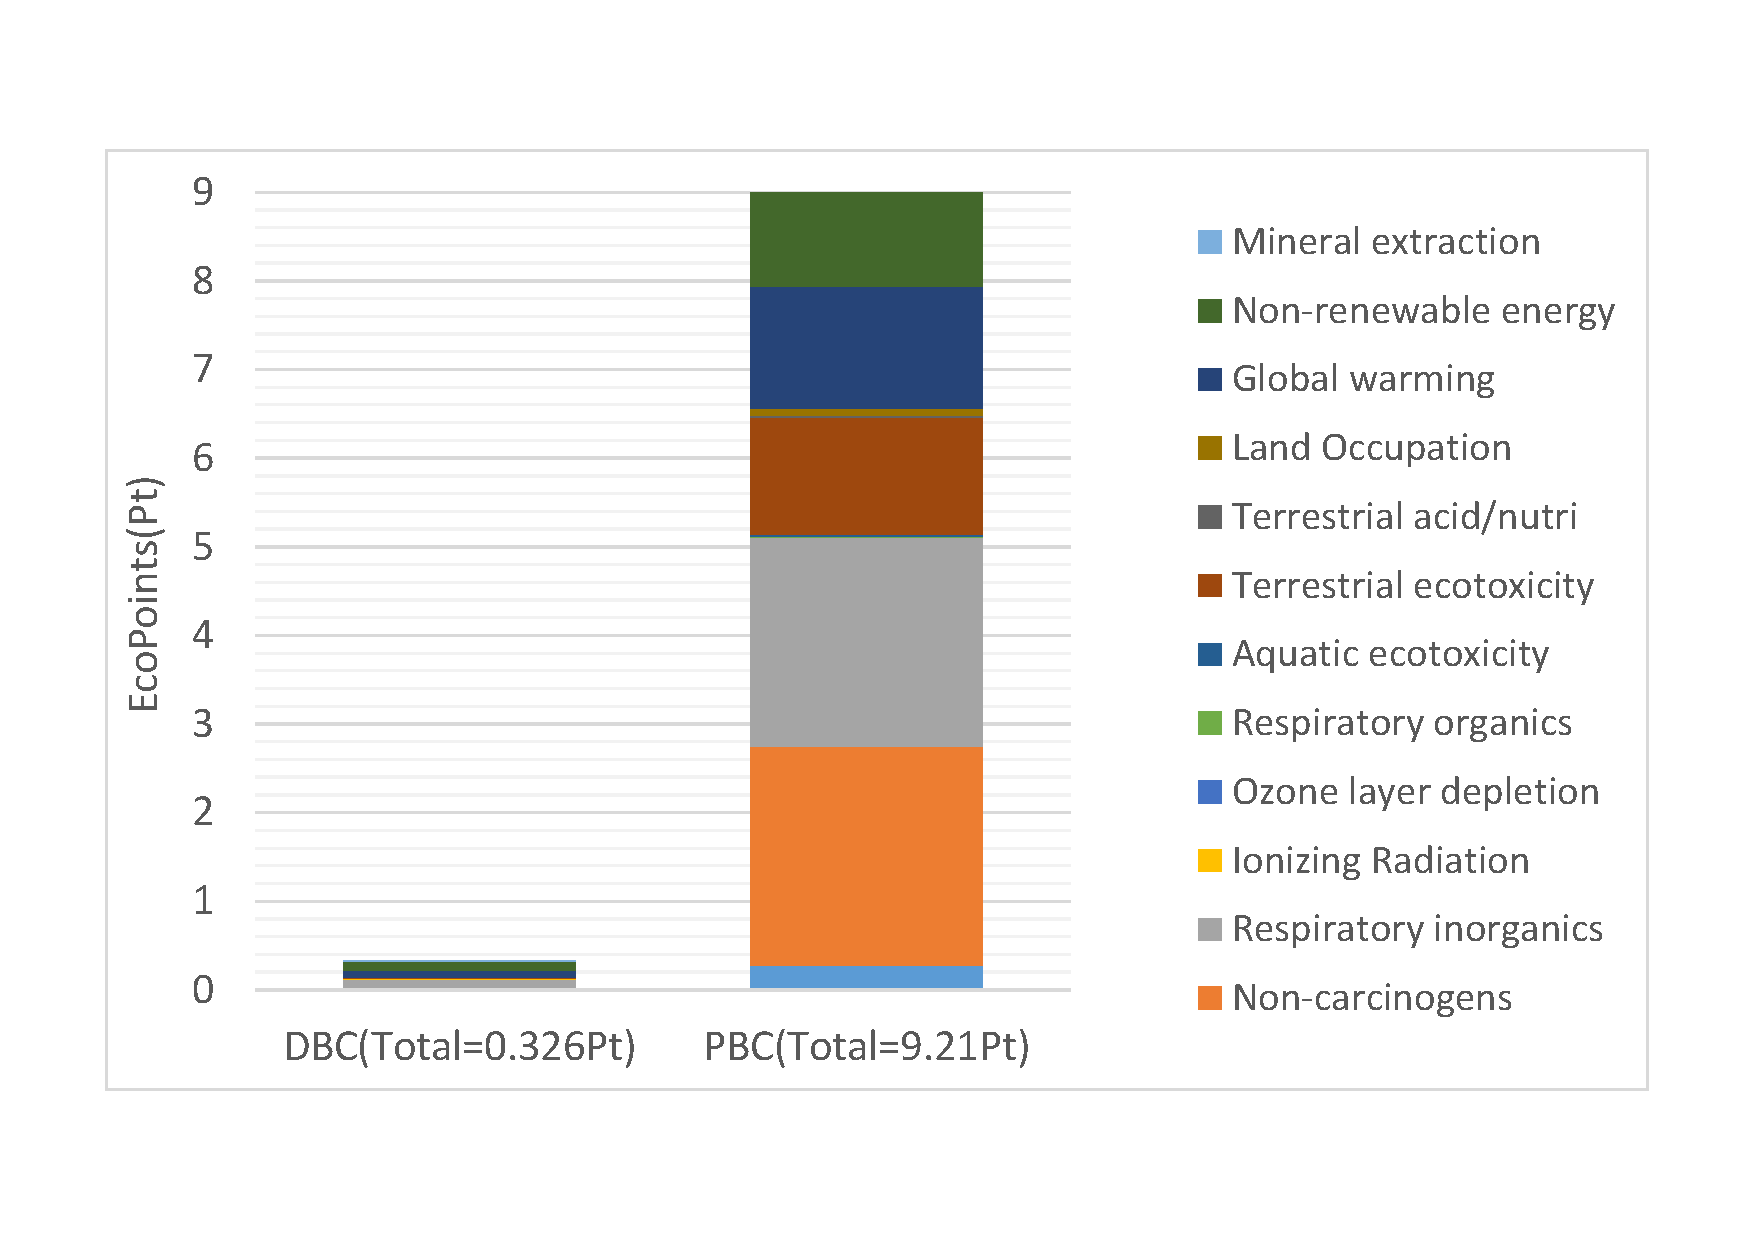
\includegraphics[width=9cm]{onescore33KMasdar.pdf}
\caption{Environmental impacts of PBC and DBC systems for 33000 exchanges in terms of Ecopoints}
\label{fig:onescoreMasdar}
\end{figure}

\end{comment}


\begin{table}[h]
\caption{Environmental impacts of PBC and DBC systems for 1000 and 33000 exchanges in terms of Ecopoints}
\centering
\begin{tabular}{ll|l|l|l|l|}
\cline{3-6}
\multicolumn{2}{l}{\multirow{2}{*}{\textbf{}}} & \multicolumn{2}{|l|}{1000 Exchnages} & \multicolumn{2}{l|}{33000 Exchanges} \\ \cline{3-6} 
\multicolumn{2}{l|}{} & DBC & PBC & DBC & PBC \\ \hline
\multicolumn{2}{|l|}{\textbf{Total}} & \textbf{0.317} & \textbf{0.279} & \textbf{0.326} & \textbf{9.21} \\ \hline
\multicolumn{2}{|l|}{Carcinogens} & 0.00106 & 0.00816 & 0.00108 & 0.0269 \\ \hline
\multicolumn{2}{|l|}{Non-carcinogens} & 0.00886 & 0.0751 & 0.00909 & 2.48 \\ \hline
\multicolumn{2}{|l|}{Respiratory inorganics} & 0.108 & 0.0713 & 0.111 & 2.35 \\ \hline
\multicolumn{2}{|l|}{Ionizing radiation} & 0.00308 & 0 & 0.00317 & 0 \\ \hline
\multicolumn{2}{|l|}{Ozone layer depletion} & 4.60E-05 & 2.11E-04 & 4.80E-05 & 0.00697 \\ \hline
\multicolumn{2}{|l|}{Respiratory organics} & 5.27E-05 & 0.000294 & 5.80E-05 & 9.72E-03 \\ \hline
\multicolumn{2}{|l|}{Aquatic ecotoxicity} & 0.00748 & 0.000651 & 0.00769 & 2.15E-02 \\ \hline
\multicolumn{2}{|l|}{Terrestrial ecotoxicity} & 0.00684 & 0.0401 & 0.00701 & 1.32 \\ \hline
\multicolumn{2}{|l|}{Terrestrial acidification} & 0.00127 & 0.00089 & 0.00131 & 0.0294 \\ \hline
\multicolumn{2}{|l|}{Land occupation} & 0.00204 & 0.00229 & 0.0021 & 0.0756 \\ \hline
\multicolumn{2}{|l|}{Global warming} & 0.0703 & 0.0415 & 0.07222 & 1.37 \\ \hline
\multicolumn{2}{|l|}{Non-renewable energy} & 0.108 & 0.0387 & 0.111 & 1.28 \\ \hline
\multicolumn{2}{|l|}{Mineral extraction} & 2.89E-04 & 0.000001918 & 2.96E-04 & 6.33E-05 \\ \hline
\end{tabular}
\label{PBCandDBCexchanges}
\end{table}




\begin{comment}
\begin{table}[htbp]

\begin{center}
\begin{tabular}{|l|r|r|}
\hline
 & \multicolumn{1}{l|}{DBC} & \multicolumn{1}{l|}{PBC} \\ \hline
Total & 0.317 & 0.279 \\ \hline
carcinogens & 0.00106 & 0.00816 \\ \hline
Non-carcinogens & 0.00886 & 0.0751 \\ \hline
Respiratory inorganics & 0.108 & 0.0713 \\ \hline
Ionizing Radiation & 0.00308 & 0 \\ \hline
Ozone layer depletion & 4.60E-05 & 2.11E-04 \\ \hline
Respiratory organics & 5.27E-05 & 0.000294 \\ \hline
Aquatic ecotoxicity & 0.00748 & 0.000651 \\ \hline
Terrestrial ecotoxicity & 0.00684 & 0.0401 \\ \hline
Terrestrial acid/nutri & 0.00127 & 0.00089 \\ \hline
Land Occupation & 0.00204 & 0.00229 \\ \hline
Global warming & 0.0703 & 0.0415 \\ \hline
Non-renewable energy & 0.108 & 0.0387 \\ \hline
Mineral extraction & 2.89E-04 & 0.000001918 \\ \hline
\end{tabular}
\end{center}
\label{PBCandDBC_2kexchanges}
\end{table}



\begin{table}[htbp]
\caption{Environmental impacts of PBC and DBC systems for 33000 exchanges in terms of Ecopoints}
\begin{center}
\begin{tabular}{|l|r|r|}
\hline
 & \multicolumn{1}{l|}{DBC} & \multicolumn{1}{l|}{PBC} \\ \hline
Total & 0.326 & 9.21 \\ \hline
carcinogens & 0.00108 & 0.0269 \\ \hline
Non-carcinogens & 0.00909 & 2.48 \\ \hline
Respiratory inorganics & 0.111 & 2.35 \\ \hline
Ionizing Radiation & 0.00317 & 0 \\ \hline
Ozone layer depletion & 4.80E-05 & 0.00697 \\ \hline
Respiratory organics & 5.80E-05 & 9.72E-03 \\ \hline
Aquatic ecotoxicity & 0.00769 & 2.15E-02 \\ \hline
Terrestrial ecotoxicity & 0.00701 & 1.32 \\ \hline
Terrestrial acid/nutri & 0.00131 & 0.0294 \\ \hline
Land Occupation & 0.0021 & 0.0756 \\ \hline
Global warming & 0.07222 & 1.37 \\ \hline
Non-renewable energy & 0.111 & 1.28 \\ \hline
Mineral extraction & 2.96E-04 & 6.33E-05 \\ \hline
\end{tabular}
\end{center}
\label{exchange_masdar}
\end{table}

\end{comment}

\section{LCIA}

Summarizing the previously shown figures, it could be noticed that different cases of functional units lead to different results. The relations between DBC and PBC systems changes in terms of environmental impact when changing the functional units. The functional unit being 1000 exchanges (i.e. 2000 cards) represents the comparison of PBC and DBC systems on the level of small sized company. As observed, the environmental impact of PBC is lower than that of DBC due to the intial high costs of the production stage of DBC system. In contrast, environmental burdens cause by DBC system are lower compared to the ones of PBC system in second and third cases i.e. functional units being 33000 and 50000 exchanges respectively. This is because the production stage of DBC system has been amortized over high number of exchanges. Moreover, the higher the number of exchanges the more amortized is the cost of the production stage.



\section{Sensitivity of Results}

A sensitivity analysis was performed having a goal of identifying parameters and assumptions that could substantially affect the results of this LCA study. According to the results life cycle burdens of the PBC and DBC systems were heavily depend on the considered assumptions and inputs. Major conclusions drawn from this analysis are detailed below.

\begin{itemize}
\item 
\item Even though the costs of a smartphone production are not considered, the impact of considering the costs of a smartphone production will result in a negligible difference. The LCA analysis of the DBC system including the cost associated with the production of smartphone is examined and provided in section. In the case of high number of exchanges, the environmental friendliness of the DBC system is not heavily dependent on the environmental effects originated from the production of smartphones.

\item PBC price upper -lower
\item numnber of exchanges affect sensitivity

\end{itemize}

\section{Conclusions}

This paper introduces a method for assessing the environmental impacts caused by DBC and PBC systems. First, screening analysis was conducted using the EIO LCA approach. This contributed to exploring the boundaries of the two systems, which in turn provided more comprehensive results. However, the variables and parameters that depend on the locality of the region could play a crucial role for determining the envoirnmental impact. In life cycle analysis, the specificity of the system studied should be preserved. Due to limitations of EIO LCA approach, these concerns were not considered while performing the screening analysis. Therefore, full LCA analyses were conducted for gaining more comprehensive and reliable results. From the conducted studies, it were observed that environmental impacts of conventional products such as newspaper and PBC and ICT enabled systems and services such as online news and DBC are difficult to assess. This is due to the multifunctionality of digital products. Given the uncertainties and obstacles posed from the latter facts, this LCA study investigates the environmental impacts of PBC and DBC systems using variable functional units. The results revealed that the number of exchanges in PBC system plays an important role in determining the environmental impact. Whereas, the manufacturing costs of the smartphone were not considered as an important contributor to the environmental burdens of DBC system. The results do not indicate that there is no environmental impact from production of smartphone. Instead, this study merely ignores the costs associated with the production of smartphone due to its infinitesimal percentage of usage by the DBC software discussed in this paper.

\section*{Acknowledgment}

This study was conducted under the support and funding of Masdar Institute of Science and Technology.

\begin{comment}
\section{Supplement Information}\label{supplement}

This section includes additional figures and tables that could be helpful for an indepth understanding of this study. Table \ref{PBCcalc} includes the monetary expense details used in the calculations in screening EIO LCA analysis. Figure \ref{onescore50K} and Table \ref{PBCandDBC50K} show the results of full LCA analysis, using Sima Pro software, having a functional unit of 50000 exchanges.

\end{comment}

\begin{comment}

\begin{figure}[h]
\centering
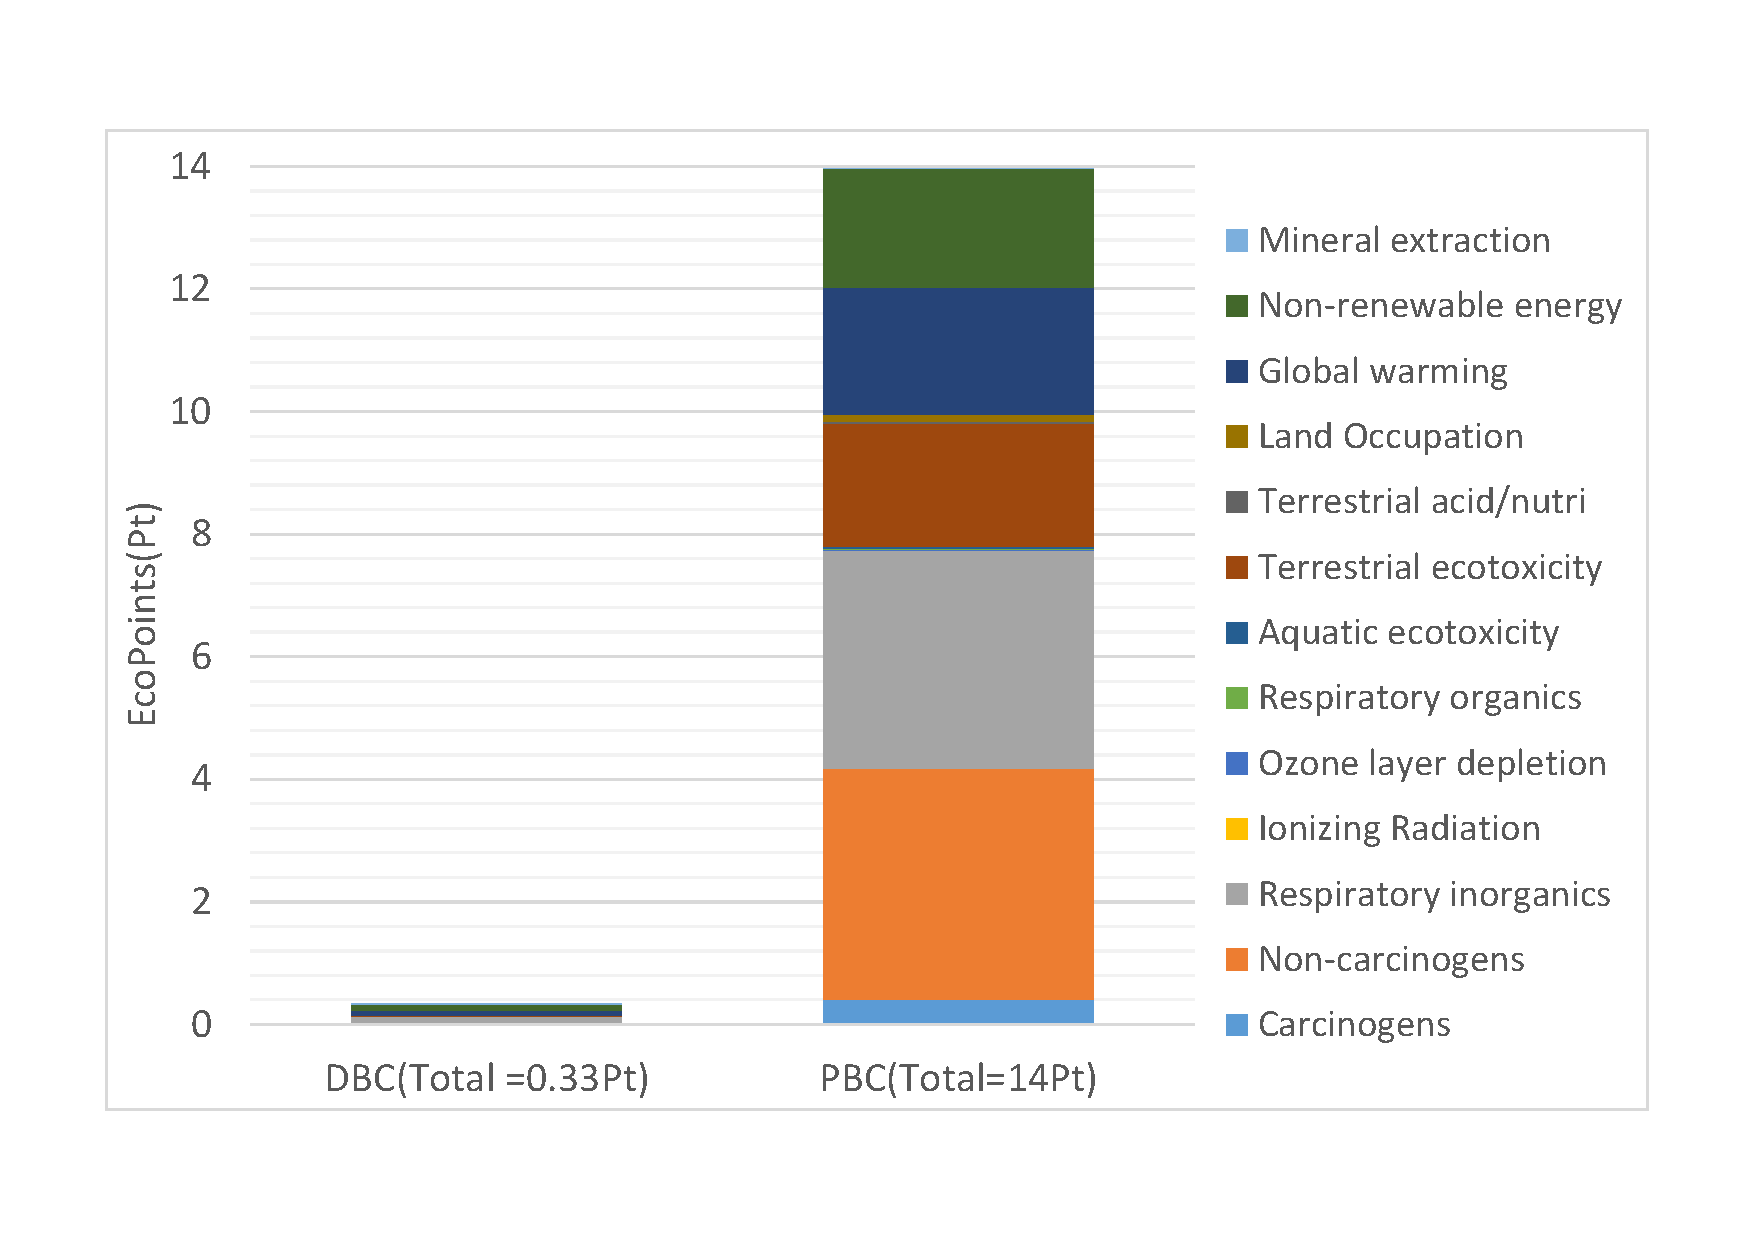
\includegraphics[width=9cm]{onescore50K.pdf}
\caption{Environmental impacts of PBC and DBC systems for 50000 exchanges in terms of Ecopoints}
\label{onescore50K}
\end{figure}



\begin{table}[htbp]
\caption{Environmental impacts of PBC and DBC systems for 50000 exchanges in terms of Ecopoints}
\begin{center}
\begin{tabular}{|l|r|r|}
\hline
 & \multicolumn{1}{l|}{PBC} & \multicolumn{1}{l|}{DBC} \\ \hline
Total & 14 & 0.33 \\ \hline
carcinogens & 0.408 & 0.00109 \\ \hline
Non-carcinogens & 3.76 & 0.00922 \\ \hline
Respiratory inorganics & 3.57 & 0.112 \\ \hline
Ionizing Radiation & 0 & 0.00322 \\ \hline
Ozone layer depletion & 0.0106 & 4.89E-05 \\ \hline
Respiratory organics & 0.0147 & 5.48E-05 \\ \hline
Aquatic ecotoxicity & 0.0325 & 0.0078 \\ \hline
Terrestrial ecotoxicity & 2 & 0.0071 \\ \hline
Terrestrial acid/nutri & 0.0445 & 0.00132 \\ \hline
Land Occupation & 0.114 & 0.00213 \\ \hline
Global warming & 2.07 & 0.0732 \\ \hline
Non-renewable energy & 1.94 & 0.112 \\ \hline
Mineral extraction & 9.59E-05 & 0.0003 \\ \hline
\end{tabular}
\end{center}
\label{PBCandDBC50K}
\end{table}

\begin{figure}[h]
\centering
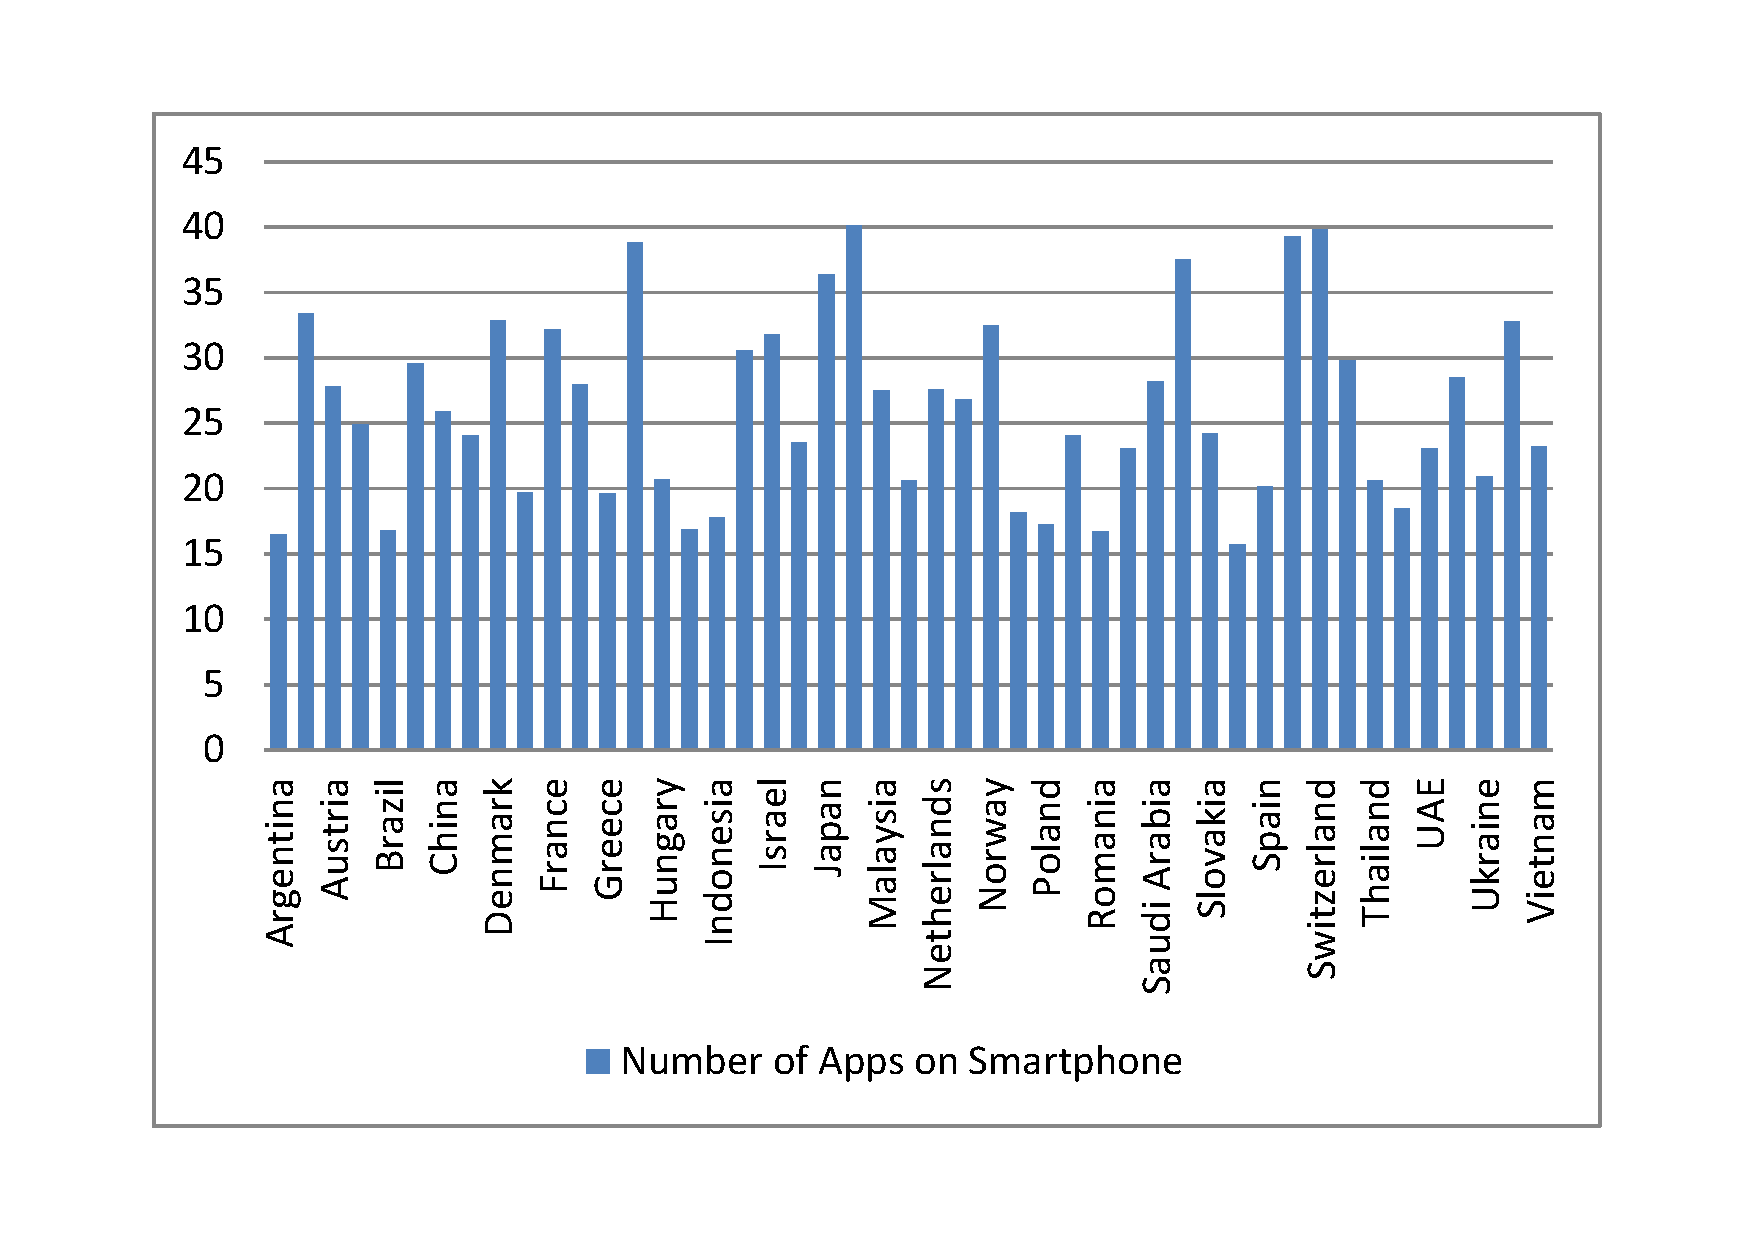
\includegraphics[width=9cm]{appsOnSmartPhone2013.pdf}
\caption{Average number of active applications used in smartphones in various countries}
\label{apps2013}
\end{figure}



\begin{table}[h]
\caption{Average number of active applications used in smartphones in 47 countries}
\begin{tabular}{|l|l|}
\hline
Country & Number of Apps on Smartphone \\ \hline
Argentina & 	16.5 \\ \hline
Australia & 	33.4 \\ \hline
Austria & 	27.8 \\ \hline
Belgium	 & 24.9 \\ \hline
Brazil & 	16.8 \\ \hline
Canada & 	29.6 \\ \hline
China & 	25.9 \\ \hline
Czech Republic & 	24.1 \\ \hline
Denmark & 	32.9 \\ \hline
Finland	 & 19.7 \\ \hline
France & 	32.2 \\ \hline
Germany	 & 28 \\ \hline
Greece	 & 19.6 \\ \hline
Hong Kong & 	38.8 \\ \hline
Hungary	 & 20.7 \\ \hline
India & 	16.9 \\ \hline
Indonesia & 	17.8 \\ \hline
Ireland & 	30.6 \\ \hline
Israel & 	31.8 \\ \hline
Italy & 	23.5 \\ \hline
Japan & 	36.4 \\ \hline
Korea & 	40.1 \\ \hline
Malaysia & 	27.5 \\ \hline
Mexico & 	20.6 \\ \hline
Netherlands & 	27.6 \\ \hline
New Zealand	 & 26.8 \\ \hline
Norway & 	32.5 \\ \hline
Philippines & 	18.2 \\ \hline
Poland & 	17.3 \\ \hline
Portugal & 	24.1 \\ \hline
Romania & 	16.7 \\ \hline
Russia & 	23.1 \\ \hline
Saudi Arabia & 	28.2 \\ \hline
Singapore & 	37.5 \\ \hline
Slovakia & 	24.2 \\ \hline
South Africa & 	15.7 \\ \hline
Spain & 	20.2 \\ \hline
Sweden & 	39.3 \\ \hline
Switzerland	 & 39.8 \\ \hline
Taiwan & 	29.8 \\ \hline
Thailand & 	20.6 \\ \hline
Turkey & 	18.5 \\ \hline
UAE	 & 23.1 \\ \hline
UK & 	28.5 \\ \hline
Ukraine	 & 20.9 \\ \hline
USA	 & 32.8 \\ \hline
Vietnam	 & 23.2 \\ \hline
Average & 26.057 \\ \hline
\label{AppTable}
\end{tabular}
\end{table}


\begin{figure}[h]
\centering
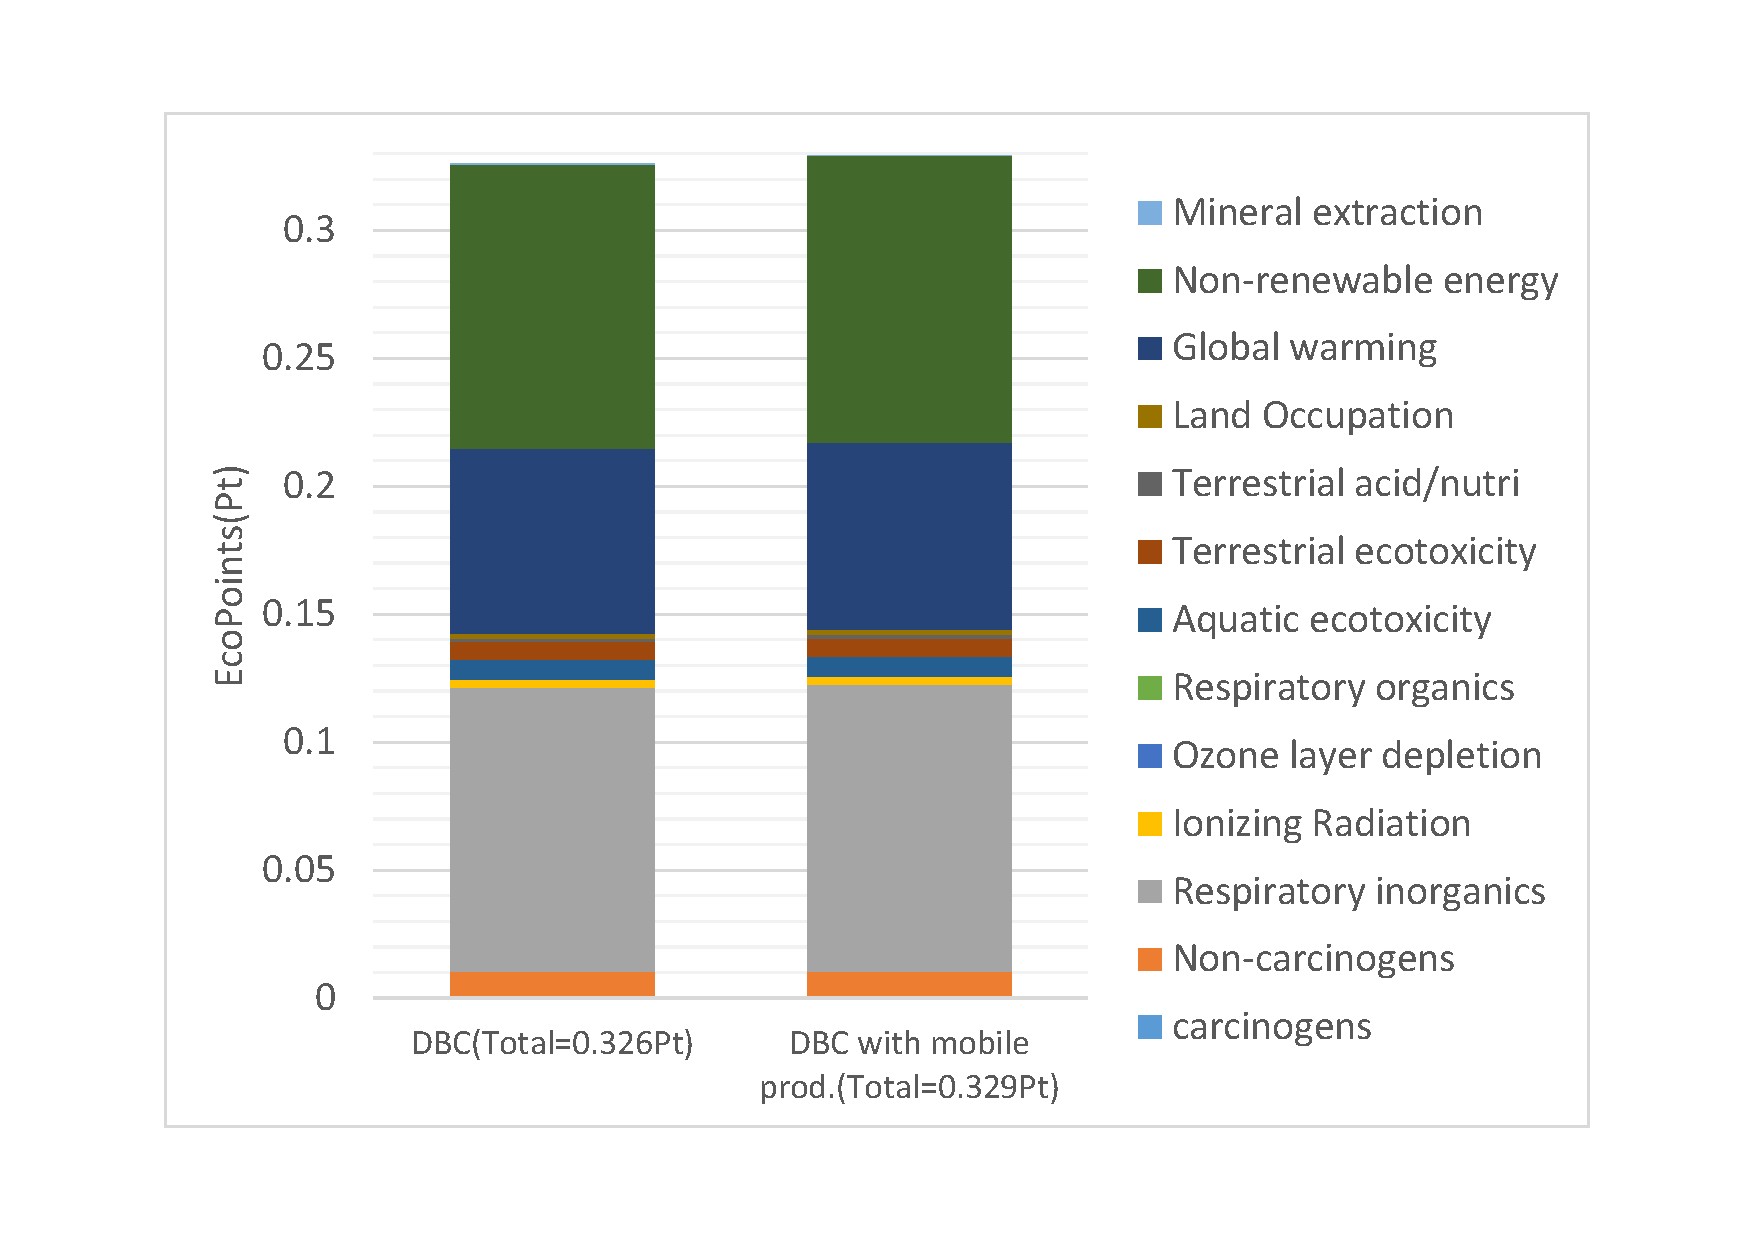
\includegraphics[width=9cm]{mobileprod.pdf}
\caption{Environmental impacts of DBC system for 33000 exchanges in terms of Ecopoints}
\label{apps2013}
\end{figure}
\end{comment}


\ifCLASSOPTIONcaptionsoff
  \newpage
\fi




% trigger a \newpage just before the given reference
% number - used to balance the columns on the last page
% adjust value as needed - may need to be readjusted if
% the document is modified later
%\IEEEtriggeratref{8}
% The "triggered" command can be changed if desired:
%\IEEEtriggercmd{\enlargethispage{-5in}}

% references section

% can use a bibliography generated by BibTeX as a .bbl file
% BibTeX documentation can be easily obtained at:
% http://www.ctan.org/tex-archive/biblio/bibtex/contrib/doc/
% The IEEEtran BibTeX style support page is at:
% http://www.michaelshell.org/tex/ieeetran/bibtex/
%\bibliographystyle{IEEEtran}
% argument is your BibTeX string definitions and bibliography database(s)
%\bibliography{IEEEabrv,../bib/paper}
%
% <OR> manually copy in the resultant .bbl file
% set second argument of \begin to the number of references
% (used to reserve space for the reference number labels box)

\bibliographystyle{plain}
\bibliography{reference}



% You can push biographies down or up by placing
% a \vfill before or after them. The appropriate
% use of \vfill depends on what kind of text is
% on the last page and whether or not the columns
% are being equalized.

%\vfill

% Can be used to pull up biographies so that the bottom of the last one
% is flush with the other column.
%\enlargethispage{-5in}




% that's all folks
\end{document}


